
Parameters + 100 elems
% CFL=0.5
% NTmaxi = 300
% length = 6.0
% ppc=1
% Nelem = 100
% E = 2.0e11
% Sigy = 400.0e6
% rho = 7800.0
% nu = 0.3
% lamb = (E*nu)/((1+nu)*(1.-2.*nu))
% mu = E/(2.*(1.+nu))
% C=lamb+2.*mu
% c=np.sqrt(C/rho)

% factor=1.
% timeOut = 1.*length/c
% t_order=1
% timeUnload = 2*timeOut

% sigd = -50.*Sigy
% v0=0.*Sigy/(rho*c)
% algo = 'USL'
% update_position=False
% mpm_mapping=True
% limit=-1
\subsection{Compression impact on a SVK medium}
\begin{figure}[h!]
  \centering
  {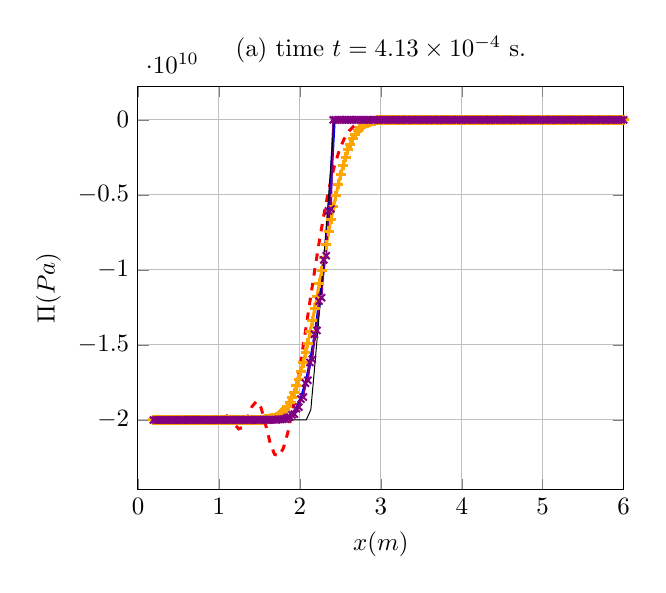
\begin{tikzpicture}[scale=0.9]
\begin{axis}[xlabel=$x (m)$,ylabel=$\Pi (Pa)$,ymajorgrids=true,xmajorgrids=true,legend pos= north west,title={(a) time $t = 4.13\times 10^{-4} $ s.},xmin=0.,xmax=6.]
\addplot[Red,very thick,mark=none,dashed] coordinates {(0.19429231621859985,-20006073362.447605) (0.2495994548763709,-19986671135.68456) (0.30488765068681783,-20009484715.95524) (0.3601633113593548,-19999667748.274166) (0.41543697640120997,-19998842866.58166) (0.4707103465207117,-19980025990.39316) (0.5259830952786003,-19989627937.11799) (0.5812473072363511,-20020206764.437843) (0.6365046678359781,-20022523341.484695) (0.6917664156560177,-19984739503.632847) (0.7470433887559937,-19921728114.52773) (0.8023244778509837,-19952983452.83056) (0.8575826939285168,-20056821377.767574) (0.9128086530876747,-20146050084.6668) (0.9680349361375865,-20050190867.486176) (1.0233128621502545,-19823950238.040665) (1.0786510045167328,-19674606159.17063) (1.1339854487171628,-19843113790.36482) (1.1892235807822906,-20263940048.802616) (1.2443383367011915,-20594817256.966568) (1.2994185016089512,-20471880070.475803) (1.3546192947754052,-19853505015.520443) (1.4100429786838058,-19090397669.844055) (1.4656431688200946,-18747034858.05499) (1.5212257963254028,-19197871377.32859) (1.5765578818799928,-20301404776.5628) (1.6315109848371214,-21504816953.264973) (1.6861313492294838,-22282313154.94336) (1.7405979869204695,-22404961380.902943) (1.795130755406773,-21893430427.415592) (1.8499225028760073,-20869875134.81481) (1.9051148450074284,-19464047060.06869) (1.9608005435269982,-17782564355.7729) (2.017033984688248,-15908990845.163458) (2.0738408016141867,-13912892750.116983) (2.1312243250448617,-11859055425.199602) (2.189169238000876,-9813911242.539871) (2.2476435755375186,-7847858230.686895) (2.306600325388235,-6032585818.503612) (2.365979745495297,-4433453223.385054) (2.425713123583109,-3098862125.3384204) (2.4857280382045643,-2050644755.106297) (2.5459543952157575,-1280061076.726812) (2.606329956594842,-751871062.4176673) (2.6668040860718976,-414991896.56532544) (2.7273390463695386,-215149915.47262502) (2.7879090497640973,-104798916.57747841) (2.8484979027936355,-47990190.44059481) (2.9090962327066574,-20674903.27414609) (2.9696990220743276,-8385318.738785009) (3.030303778267326,-3203330.0276726247) (3.0909093485437626,-1152979.973410103) (3.151515235363365,-391035.675115866) (3.2121212378932866,-124947.32039185325) (3.272727280203827,-37601.22723226968) (3.333333335378876,-10651.218022956937) (3.393939394466688,-2837.8277527031114) (3.454545454673374,-710.4571418349901) (3.515151515180682,-166.93032426436852) (3.5757575757638156,-36.758497954882436) (3.6363636363648877,-7.573117346901461) (3.6969696969699313,-1.456928594861368) (3.7575757575757986,-0.2611244553918368) (3.8181818181818246,-0.043490851945412384) (3.87878787878788,-0.006695498856200944) (3.9393939393939394,-0.000956499836600135) (4.0,-0.00011956247957501687) (4.0606060606060606,0.0) (4.121212121212121,0.0) (4.181818181818182,0.0) (4.242424242424242,0.0) (4.303030303030303,0.0) (4.363636363636363,0.0) (4.424242424242425,0.0) (4.484848484848485,0.0) (4.545454545454546,0.0) (4.606060606060606,0.0) (4.666666666666667,0.0) (4.7272727272727275,0.0) (4.787878787878788,0.0) (4.848484848484849,0.0) (4.909090909090909,0.0) (4.96969696969697,0.0) (5.03030303030303,0.0) (5.090909090909091,0.0) (5.151515151515151,0.0) (5.212121212121212,0.0) (5.2727272727272725,0.0) (5.333333333333334,0.0) (5.3939393939393945,0.0) (5.454545454545455,0.0) (5.515151515151516,0.0) (5.575757575757576,0.0) (5.636363636363637,0.0) (5.696969696969697,0.0) (5.757575757575758,0.0) (5.818181818181818,0.0) (5.878787878787879,0.0) (5.9393939393939394,0.0) (6.0,0.0) };
\addplot[Blue,very thick,mark=none,solid] coordinates {(0.19184481823272587,-20000746788.895386) (0.2472984593148165,-19999262845.167934) (0.3027550579515747,-20000799959.541138) (0.3582139828028267,-19999230865.055157) (0.4136744334611789,-20000901266.778095) (0.4691363798583578,-19999156573.758553) (0.5245991019399393,-20001058323.113438) (0.5800629488714097,-19999036648.84517) (0.635527105553384,-20001282242.769444) (0.6909922402572966,-19998864927.72781) (0.7464573416593343,-20001588390.21625) (0.8019234043904636,-19998632043.305565) (0.8573891369717147,-20001997440.71843) (0.9128559063396893,-19998324890.49686) (0.9683220513996212,-20002536843.16476) (1.023789388354951,-19997925908.97679) (1.0792557790732065,-20003242807.18485) (1.1347235977259633,-19997412156.041016) (1.1901900940405064,-20004162964.68389) (1.2456583458259118,-19996754091.63044) (1.3011248178858221,-20005359727.42986) (1.3565934830124184,-19995913073.930134) (1.412059799077113,-20006909700.64143) (1.467528884562971,-19994813482.07538) (1.5229949116205286,-20008792500.146915) (1.5784645009572125,-19992861846.161507) (1.63393029649414,-20009157097.143948) (1.689401269313731,-19983335218.807507) (1.7448693336716496,-19988556060.043617) (1.8003496405947086,-19915211430.44971) (1.8558399943620645,-19832464370.455975) (1.9113756485372175,-19565996896.830357) (1.9669788598771232,-19175060421.84385) (2.022726722440876,-18428718648.265965) (2.078678157853173,-17432821776.53043) (2.134949207911814,-15950492705.79851) (2.191612836208383,-14179637125.40624) (2.248793446466984,-11863860055.04507) (2.3065513731895595,-9241855726.717867) (2.365009406439806,-5893766492.953189) (2.4242424242424243,0.0) (2.484848484848485,0.0) (2.5454545454545454,0.0) (2.606060606060606,0.0) (2.666666666666667,0.0) (2.7272727272727275,0.0) (2.787878787878788,0.0) (2.8484848484848486,0.0) (2.909090909090909,0.0) (2.9696969696969697,0.0) (3.0303030303030303,0.0) (3.090909090909091,0.0) (3.1515151515151514,0.0) (3.2121212121212124,0.0) (3.272727272727273,0.0) (3.3333333333333335,0.0) (3.393939393939394,0.0) (3.4545454545454546,0.0) (3.515151515151515,0.0) (3.5757575757575757,0.0) (3.6363636363636367,0.0) (3.6969696969696972,0.0) (3.757575757575758,0.0) (3.8181818181818183,0.0) (3.878787878787879,0.0) (3.9393939393939394,0.0) (4.0,0.0) (4.0606060606060606,0.0) (4.121212121212121,0.0) (4.181818181818182,0.0) (4.242424242424242,0.0) (4.303030303030303,0.0) (4.363636363636363,0.0) (4.424242424242425,0.0) (4.484848484848485,0.0) (4.545454545454546,0.0) (4.606060606060606,0.0) (4.666666666666667,0.0) (4.7272727272727275,0.0) (4.787878787878788,0.0) (4.848484848484849,0.0) (4.909090909090909,0.0) (4.96969696969697,0.0) (5.03030303030303,0.0) (5.090909090909091,0.0) (5.151515151515151,0.0) (5.212121212121212,0.0) (5.2727272727272725,0.0) (5.333333333333334,0.0) (5.3939393939393945,0.0) (5.454545454545455,0.0) (5.515151515151516,0.0) (5.575757575757576,0.0) (5.636363636363637,0.0) (5.696969696969697,0.0) (5.757575757575758,0.0) (5.818181818181818,0.0) (5.878787878787879,0.0) (5.9393939393939394,0.0) (6.0,0.0) };
\addplot[Orange,very thick,mark=+,solid] coordinates {(0.18995525166111366,-19999912858.22518) (0.21763857805956868,-19999769787.88829) (0.24512208706281055,-19999595225.830395) (0.27282575705740886,-19999451694.173355) (0.3003071750929951,-19999276292.69227) (0.32801595744355366,-19999131832.277004) (0.3554953427946694,-19998955018.611973) (0.3832066011773739,-19998809148.97717) (0.4106846406234849,-19998630330.553932) (0.4383974367587157,-19998482551.158222) (0.46587453401796425,-19998301106.73408) (0.49358840901570517,-19998150889.20853) (0.5210648104045611,-19997966159.024174) (0.5487795002679247,-19997812938.436954) (0.5762553672290964,-19997624212.983093) (0.6039707041588833,-19997467377.749435) (0.6314461490108538,-19997273884.659058) (0.659162018895618,-19997112764.632294) (0.6866371235984735,-19996913653.070396) (0.7143534449920753,-19996747505.207943) (0.7418282717305508,-19996541826.930435) (0.7695449843941599,-19996369817.725258) (0.7970195819297244,-19996156503.688694) (0.8247366401192712,-19995977687.259945) (0.8522110478099802,-19995755518.23956) (0.8799284161209588,-19995568808.532024) (0.9074026665852393,-19995336377.560326) (0.9351203172698606,-19995140512.397816) (0.9625944382274981,-19994896175.737343) (0.9903123494081251,-19994689669.049244) (1.0177863650063577,-19994431479.734898) (1.0455045194632855,-19994212553.503006) (1.0729784512767135,-19993938160.470367) (1.1006968356268219,-19993704624.606678) (1.1281707034621382,-19993411064.120533) (1.1558893076415115,-19993159994.96435) (1.1833631302893026,-19992843029.618053) (1.2110819473987793,-19992569575.424583) (1.2385557436795793,-19992221110.35909) (1.2662747707021536,-19991913792.57851) (1.2937485620273468,-19991511992.659107) (1.3214678034398997,-19991135778.789246) (1.348941622020031,-19990611361.07096) (1.3766611027821543,-19990054404.717606) (1.4041350176396072,-19989191087.10363) (1.43185482298986,-19988120795.17056) (1.4593290140068589,-19986303943.14754) (1.4870493950945292,-19983836663.36228) (1.5145243372708168,-19979517453.333805) (1.5422459535049426,-19973584795.21019) (1.5697228130621068,-19963335295.939476) (1.5974472092249048,-19949696944.16045) (1.6249285708236694,-19926887514.67977) (1.6526589729400751,-19897960308.693275) (1.6801499595587883,-19851437924.117283) (1.7078923745712826,-19795437569.700573) (1.7354020457070085,-19708969482.813923) (1.7631664627875865,-19610053565.1548) (1.7907091203275556,-19463351503.24422) (1.8185104215571681,-19303209212.943596) (1.846106271632855,-19074774470.23491) (1.8739644155740336,-18835426807.336002) (1.9016391139595983,-18506490966.59541) (1.929578344685977,-18173408100.377052) (1.9573613220878685,-17731609002.064552) (1.9854084938213,-17296152224.080425) (2.013330410494915,-16737796934.560286) (2.041512798178765,-16198491879.856827) (2.069602736105936,-15529090279.041159) (2.097945774544229,-14891880186.885708) (2.1262287257995864,-14125409710.52269) (2.154753998432247,-13403375220.585518) (2.1832489573267595,-12561011287.379313) (2.211972566392059,-11773975414.023428) (2.24069126999827,-10882817742.279064) (2.2696225838776267,-10056933247.623539) (2.2985687962945347,-9148834985.540192) (2.327709541119762,-8315860661.742456) (2.356878766471977,-7426050359.213425) (2.3862225001407333,-6621710808.248219) (2.4156021007706037,-5786632187.628343) (2.4451342315442015,-5047407133.728801) (2.47470405839892,-4301249043.455953) (2.5044026660566034,-3659402379.111651) (2.5341363952031912,-3029346440.874573) (2.563974070845136,-2507081699.0016084) (2.593841384344465,-2008351349.8441858) (2.623788042880702,-1613201600.0153964) (2.6537575319704074,-1245972269.7087686) (2.6837837243855356,-969806805.9692637) (2.713826006898169,-719895044.9301026) (2.743905915736818,-542465644.1033932) (2.773996200748826,-386006963.2538726) (2.804109532245024,-281510641.82021976) (2.8342289849581657,-191643401.31466892) (2.8643614213299275,-135290962.20125788) (2.8944971613083075,-87983443.40475516) (2.924639617951817,-60153986.76079956) (2.9547837066305997,-37328498.31375421) (2.9849309849010037,-24733077.95371384) (3.015079001851262,-14631759.500679849) (3.045228409801474,-9402072.941124339) (3.0753781243862,-5298061.620119785) (3.105528396475034,-3304104.722537816) (3.1356787854200334,-1771954.9486091677) (3.1658293798711896,-1073279.4290237231) (3.195980015238912,-547296.2783473512) (3.226130720321594,-322187.11395850533) (3.2562814385751238,-156061.14816243792) (3.286432178602333,-89350.21257776454) (3.316582922528392,-41065.456399169176) (3.3467336727166184,-22880.71737255304) (3.3768844239662927,-9965.667379406394) (3.4070351768743565,-5407.004064866737) (3.437185930048142,-2228.6748053008914) (3.4673366836262214,-1178.1706413573809) (3.497487437265445,-458.856763768479) (3.527638190995354,-236.47913094118658) (3.5577889447381867,-86.87293189700003) (3.587939698499721,-43.6702853295511) (3.618090452263762,-15.102474825431294) (3.6482412060313454,-7.4089580622410764) (3.6783919597993746,-2.406673151344001) (3.7085427135680193,-1.1526420843380152) (3.7386934673367365,-0.35061697135328035) (3.768844221105552,-0.1639201594972483) (3.798994974874379,-0.04639024207509855) (3.8291457286432187,-0.02113266826488257) (3.8592964824120606,-0.005410202200769404) (3.8894472361809047,-0.002271687111925301) (3.9195979899497484,-0.00044835929840631247) (3.949748743718593,-0.00017934371936252516) (3.979899497487437,0.0) (4.010050251256281,0.0) (4.040201005025126,0.0) (4.0703517587939695,0.0) (4.100502512562814,0.0) (4.130653266331658,-5.9781239787508415e-05) (4.160804020100502,0.0) (4.190954773869347,0.0) (4.221105527638191,0.0) (4.251256281407035,0.0) (4.281407035175879,0.0) (4.311557788944723,0.0) (4.341708542713568,0.0) (4.371859296482412,0.0) (4.402010050251256,0.0) (4.4321608040201,-5.9781239787508415e-05) (4.4623115577889445,0.0) (4.492462311557789,0.0) (4.522613065326633,0.0) (4.552763819095477,0.0) (4.582914572864321,0.0) (4.613065326633166,0.0) (4.64321608040201,0.0) (4.673366834170854,0.0) (4.703517587939698,0.0) (4.733668341708542,0.0) (4.763819095477387,0.0) (4.793969849246231,0.0) (4.824120603015075,0.0) (4.8542713567839195,0.0) (4.884422110552763,0.0) (4.914572864321608,0.0) (4.944723618090452,0.0) (4.974874371859296,0.0) (5.005025125628141,0.0) (5.035175879396984,0.0) (5.065326633165829,0.0) (5.0954773869346734,0.0) (5.125628140703517,0.0) (5.155778894472362,0.0) (5.185929648241205,0.0) (5.21608040201005,0.0) (5.2462311557788945,0.0) (5.276381909547738,-5.9781239787508415e-05) (5.306532663316583,0.0) (5.3366834170854265,0.0) (5.366834170854271,0.0) (5.396984924623116,0.0) (5.427135678391959,0.0) (5.457286432160804,0.0) (5.487437185929648,0.0) (5.517587939698492,0.0) (5.547738693467337,0.0) (5.57788944723618,0.0) (5.608040201005025,0.0) (5.638190954773869,-5.9781239787508415e-05) (5.668341708542713,0.0) (5.698492462311558,0.0) (5.7286432160804015,0.0) (5.758793969849246,0.0) (5.788944723618091,0.0) (5.819095477386934,0.0) (5.849246231155779,0.0) (5.879396984924623,-5.9781239787508415e-05) (5.909547738693467,0.0) (5.939698492462312,0.0) (5.969849246231155,0.0) (6.0,0.0) };
\addplot[Purple,thick,mark=x,solid] coordinates {(0.19087078866902665,-19999455640.176197) (0.22071218292775385,-19999409659.864017) (0.2459924077656396,-20000077312.85232) (0.27597326522813487,-20000072009.997063) (0.3011894927456019,-19998950742.164944) (0.3311766255539742,-19998862763.515118) (0.3563962430072859,-19999589159.90041) (0.38636963567121163,-19999626165.686943) (0.41160234396465,-19998404877.00223) (0.4415609586628959,-19998270520.060898) (0.4668064289385858,-19999118873.727676) (0.49675180124731944,-19999202922.963924) (0.5220088990140508,-19997806766.43407) (0.5519428363462726,-19997618279.35031) (0.5772098159593475,-19998661098.62433) (0.6071336614902496,-19998800403.628937) (0.6324097933704171,-19997141589.490086) (0.6623248466555562,-19996887265.347076) (0.6876086367678674,-19998211885.709827) (0.7175157537096876,-19998418772.38764) (0.7428070060201625,-19996389972.392735) (0.7727071471896477,-19996053259.198273) (0.7980044513100885,-19997768502.897907) (0.8278981543338224,-19998060358.486023) (0.8532017639590902,-19995526549.26538) (0.8830898001721301,-19995084778.141758) (0.9083982334111295,-19997329243.71315) (0.9382809151671918,-19997729846.142517) (0.9635948605946703,-19994517924.97995) (0.9934728615949118,-19993940550.927967) (1.018790634157661,-19996893154.38264) (1.0486640867664065,-19997434481.72408) (1.0739868482392012,-19993319799.35868) (1.103856391967528,-19992566008.07375) (1.129182120960812,-19996459571.531334) (1.1590477257284901,-19997184225.495197) (1.1843781409943626,-19991872941.060112) (1.2142404634066721,-19990888423.449177) (1.2395730548989103,-19996027394.59501) (1.269431901039365,-19996991817.22908) (1.2947690752904193,-19990097771.00673) (1.3246251669949154,-19988810395.611206) (1.3499637385624637,-19995594394.611435) (1.3798167010879285,-19996873032.549503) (1.4051599499623135,-19987887684.922043) (1.4350106214725087,-19986201196.541973) (1.4603544495160277,-19995154760.05428) (1.4902022422851016,-19996842075.848194) (1.5155510581278278,-19985077422.35594) (1.5453969866641184,-19982845663.359066) (1.570745480163516,-19994550689.773247) (1.6005886999258214,-19996684108.793686) (1.625942792905406,-19980692933.116657) (1.6557845912583171,-19977385747.898075) (1.6811375441326768,-19990452521.34305) (1.7109768445952687,-19991936790.38711) (1.736337222388458,-19962562834.670414) (1.7661759691627483,-19954268934.61151) (1.7915371396346151,-19946636578.575214) (1.8213747099598598,-19938461812.41097) (1.8467537764093123,-19837157162.833206) (1.8765945013072705,-19804712010.78006) (1.9019952765295465,-19662159771.99237) (1.9318415620560758,-19612768170.56989) (1.9573086438181697,-19243797603.25251) (1.987170301328827,-19145197075.79308) (2.0127391582847944,-18606422582.842396) (2.042623150182732,-18474857956.820774) (2.068383513683698,-17546640829.370613) (2.0983030697861436,-17356604515.480618) (2.1243218125728434,-16168446386.224903) (2.154282226835199,-15957833195.666677) (2.1806765607592036,-14287253493.297613) (2.2106861953891266,-14032581607.352451) (2.2375256180290903,-12078287603.813477) (2.2675794640427664,-11846950370.664488) (2.2949840954789456,-9331938813.91532) (2.325083226953284,-9055544632.420107) (2.3531208903662257,-6074271277.8443) (2.3832414203422285,-5944142832.467713) (2.4120603015075375,0.0004184686785125597) (2.4422110552763816,0.0004184686785125597) (2.472361809045226,0.000717374877450103) (2.5025125628140703,0.000717374877450103) (2.5326633165829144,0.0001793437193625254) (2.5628140703517586,0.0001793437193625254) (2.5929648241206027,0.0005978123978750856) (2.6231155778894473,0.0005978123978750856) (2.6532663316582914,0.0005978123978750856) (2.6834170854271355,0.0005978123978750856) (2.7135678391959797,0.0006575936376625943) (2.743718592964824,0.0005978123978750856) (2.7738693467336684,0.0005380311580875769) (2.8040201005025125,0.0004782499183000683) (2.8341708542713566,0.0003586874387250511) (2.8643216080402008,0.0003586874387250511) (2.8944723618090453,0.00011956247957501691) (2.9246231155778895,0.00011956247957501691) (2.9547738693467336,0.0005380311580875769) (2.9849246231155777,0.0004782499183000683) (3.015075376884422,0.0005380311580875769) (3.0452261306532664,0.0005380311580875769) (3.0753768844221105,0.000717374877450103) (3.1055276381909547,0.000717374877450103) (3.135678391959799,0.0001793437193625254) (3.165829145728643,0.00011956247957501691) (3.1959798994974875,0.0005978123978750856) (3.2261306532663316,0.0005978123978750856) (3.2562814070351758,0.0004782499183000683) (3.28643216080402,0.0004782499183000683) (3.316582914572864,0.0002989061989375425) (3.3467336683417086,0.00023912495915003393) (3.3768844221105527,0.0005978123978750856) (3.407035175879397,0.0005380311580875769) (3.437185929648241,0.0004184686785125597) (3.467336683417085,0.0004184686785125597) (3.4974874371859297,0.0002989061989375425) (3.527638190954774,0.0002989061989375425) (3.557788944723618,5.978123978750844e-05) (3.587939698492462,5.978123978750844e-05) (3.618090452261306,0.00011956247957501691) (3.648241206030151,0.0) (3.678391959798995,0.0001793437193625254) (3.708542713567839,0.00011956247957501691) (3.738693467336683,0.0005978123978750856) (3.7688442211055273,0.0005978123978750856) (3.798994974874372,0.0) (3.829145728643216,-0.0001195624795750168) (3.85929648241206,0.0003586874387250511) (3.8894472361809043,0.0002989061989375425) (3.9195979899497484,0.0004782499183000683) (3.949748743718593,0.0004782499183000683) (3.979899497487437,0.00011956247957501691) (4.010050251256281,5.978123978750844e-05) (4.040201005025126,-0.00032879681883129597) (4.0703517587939695,-0.00032879681883129597) (4.100502512562814,0.0005978123978750856) (4.130653266331658,0.0005978123978750856) (4.160804020100502,0.0) (4.190954773869347,0.00011956247957501691) (4.221105527638191,0.0005978123978750856) (4.251256281407035,0.0005978123978750856) (4.281407035175879,0.00023912495915003393) (4.311557788944723,0.00023912495915003393) (4.341708542713568,-5.9781239787508415e-05) (4.371859296482412,-0.0001195624795750168) (4.402010050251256,0.0005978123978750856) (4.4321608040201,0.0005978123978750856) (4.4623115577889445,-0.00044835929840631247) (4.492462311557789,-0.00044835929840631247) (4.522613065326633,0.0004782499183000683) (4.552763819095477,0.0005380311580875769) (4.582914572864321,0.0001793437193625254) (4.613065326633166,0.00011956247957501691) (4.64321608040201,0.0005978123978750856) (4.673366834170854,0.0005380311580875769) (4.703517587939698,0.0006575936376625943) (4.733668341708542,0.0006575936376625943) (4.763819095477387,-0.00032879681883129597) (4.793969849246231,-0.00032879681883129597) (4.824120603015075,0.0005978123978750856) (4.8542713567839195,0.0005978123978750856) (4.884422110552763,-0.00029890619893754183) (4.914572864321608,-0.00029890619893754183) (4.944723618090452,0.0006575936376625943) (4.974874371859296,0.0005978123978750856) (5.005025125628141,-0.00032879681883129597) (5.035175879396984,-0.00032879681883129597) (5.065326633165829,0.00023912495915003393) (5.0954773869346734,0.00023912495915003393) (5.125628140703517,0.0003586874387250511) (5.155778894472362,0.0004184686785125597) (5.185929648241205,-0.00044835929840631247) (5.21608040201005,-0.00032879681883129597) (5.2462311557788945,0.0005978123978750856) (5.276381909547738,0.0005978123978750856) (5.306532663316583,0.00023912495915003393) (5.3366834170854265,0.00023912495915003393) (5.366834170854271,-0.00044835929840631247) (5.396984924623116,-0.0003885780586188042) (5.427135678391959,0.0003586874387250511) (5.457286432160804,0.0004184686785125597) (5.487437185929648,-0.0003885780586188042) (5.517587939698492,-0.00044835929840631247) (5.547738693467337,0.0005978123978750856) (5.57788944723618,0.0005978123978750856) (5.608040201005025,-0.00029890619893754183) (5.638190954773869,-0.00029890619893754183) (5.668341708542713,0.0006575936376625943) (5.698492462311558,0.0006575936376625943) (5.7286432160804015,-0.00017934371936252516) (5.758793969849246,-0.00017934371936252516) (5.788944723618091,-0.00032879681883129597) (5.819095477386934,-0.00032879681883129597) (5.849246231155779,0.0006575936376625943) (5.879396984924623,0.0006575936376625943) (5.909547738693467,-0.00032879681883129597) (5.939698492462312,-0.00032879681883129597) (5.969849246231155,0.0011358435559626649) (6.0,0.0007771561172376117) };
\addplot[black,thin,mark=none,solid] coordinates {(0.19184481823272587,-19999999999.99513) (0.2472984593148165,-19999999999.99513) (0.3027550579515747,-19999999999.99513) (0.3582139828028267,-19999999999.99513) (0.4136744334611789,-19999999999.99513) (0.4691363798583578,-19999999999.99513) (0.5245991019399393,-19999999999.99513) (0.5800629488714097,-19999999999.99513) (0.635527105553384,-19999999999.99513) (0.6909922402572966,-19999999999.99513) (0.7464573416593343,-19999999999.99513) (0.8019234043904636,-19999999999.99513) (0.8573891369717147,-19999999999.99513) (0.9128559063396893,-19999999999.99513) (0.9683220513996212,-19999999999.99513) (1.023789388354951,-19999999999.99513) (1.0792557790732065,-19999999999.99513) (1.1347235977259633,-19999999999.99513) (1.1901900940405064,-19999999999.99513) (1.2456583458259118,-19999999999.99513) (1.3011248178858221,-19999999999.99513) (1.3565934830124184,-19999999999.99513) (1.412059799077113,-19999999999.99513) (1.467528884562971,-19999999999.99513) (1.5229949116205286,-19999999999.99513) (1.5784645009572125,-19999999999.99513) (1.63393029649414,-19999999999.99513) (1.689401269313731,-19999999999.99513) (1.7448693336716496,-19999999999.99513) (1.8003496405947086,-19999999999.99513) (1.8558399943620645,-19999999999.99513) (1.9113756485372175,-19999999999.99513) (1.9669788598771232,-19999999999.99513) (2.022726722440876,-19999999999.99513) (2.078678157853173,-19999999999.99513) (2.134949207911814,-19320644756.027233) (2.191612836208383,-15934816130.431961) (2.248793446466984,-12317415446.21064) (2.3065513731895595,-8460847327.543606) (2.365009406439806,-4357551166.693738) (2.4242424242424243,-8.967185968126261e-05) (2.484848484848485,0.0) (2.5454545454545454,0.0) (2.606060606060606,0.0) (2.666666666666667,0.0) (2.7272727272727275,0.0) (2.787878787878788,0.0) (2.8484848484848486,0.0) (2.909090909090909,0.0) (2.9696969696969697,0.0) (3.0303030303030303,0.0) (3.090909090909091,0.0) (3.1515151515151514,0.0) (3.2121212121212124,0.0) (3.272727272727273,0.0) (3.3333333333333335,0.0) (3.393939393939394,0.0) (3.4545454545454546,0.0) (3.515151515151515,0.0) (3.5757575757575757,0.0) (3.6363636363636367,0.0) (3.6969696969696972,0.0) (3.757575757575758,0.0) (3.8181818181818183,0.0) (3.878787878787879,0.0) (3.9393939393939394,0.0) (4.0,0.0) (4.0606060606060606,0.0) (4.121212121212121,0.0) (4.181818181818182,0.0) (4.242424242424242,0.0) (4.303030303030303,0.0) (4.363636363636363,0.0) (4.424242424242425,0.0) (4.484848484848485,0.0) (4.545454545454546,0.0) (4.606060606060606,0.0) (4.666666666666667,0.0) (4.7272727272727275,0.0) (4.787878787878788,0.0) (4.848484848484849,0.0) (4.909090909090909,0.0) (4.96969696969697,0.0) (5.03030303030303,0.0) (5.090909090909091,0.0) (5.151515151515151,0.0) (5.212121212121212,0.0) (5.2727272727272725,0.0) (5.333333333333334,0.0) (5.3939393939393945,0.0) (5.454545454545455,0.0) (5.515151515151516,0.0) (5.575757575757576,0.0) (5.636363636363637,0.0) (5.696969696969697,0.0) (5.757575757575758,0.0) (5.818181818181818,0.0) (5.878787878787879,0.0) (5.9393939393939394,0.0) (6.0,0.0) };
%\legend{mpm,dgmpm,dgmpm 2ppc,dgmpm 2ppc (RK2),exact}
\end{axis}
\end{tikzpicture}
%%% Local Variables:
%%% mode: latex
%%% TeX-master: "../../mainManuscript"
%%% End:
}
  {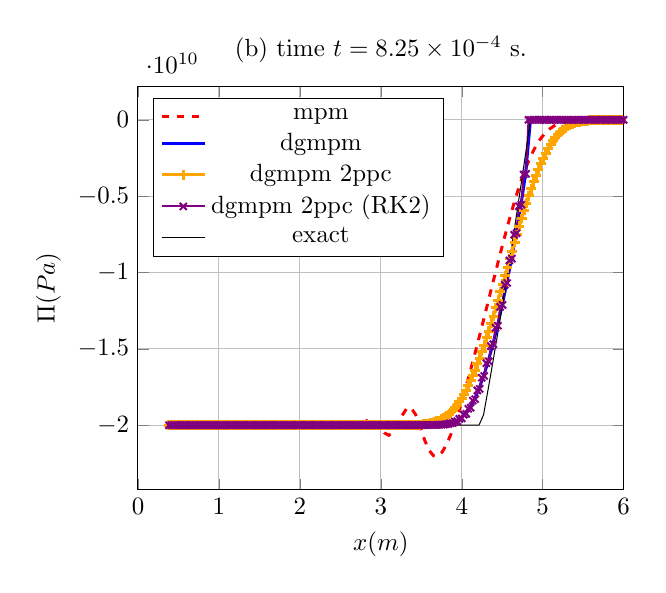
\begin{tikzpicture}[scale=0.9]
\begin{axis}[xlabel=$x (m)$,ylabel=$\Pi (Pa)$,ymajorgrids=true,xmajorgrids=true,legend pos= north west,title={(b) time $t = 8.25\times 10^{-4} $ s.},xmin=0.,xmax=6.]
\addplot[Red,very thick,mark=none,dashed] coordinates {(0.39037665296779944,-20003189832.924717) (0.4456826624098611,-19996503392.149483) (0.5009704081817377,-20002423865.30926) (0.5562477051357223,-19996663831.661327) (0.6115214671319547,-20001250436.505577) (0.6667916713890001,-19997098449.727352) (0.7220599841425713,-19999850425.379917) (0.7773261888093733,-19997733483.30031) (0.8325911169429844,-19998457405.552814) (0.8878545954294681,-19998172379.55476) (0.9431171523187737,-19997060791.85406) (0.9983786116645804,-19998515112.86419) (1.0536392800775984,-19996294129.02629) (1.1088991050268924,-19998580900.381916) (1.1641583617305475,-19995161992.177692) (1.2194170584909185,-19997783430.157677) (1.2746751455719256,-19995019664.29004) (1.3299325546069887,-19998356312.732986) (1.3851894014031947,-19995142276.615314) (1.440446120748,-19996033685.0159) (1.4957027682981452,-19992681848.43269) (1.5509590057181089,-19995837672.158688) (1.6062141479872896,-19996864692.176643) (1.6614684602296836,-19998537719.943672) (1.7167230488688772,-19992892483.20531) (1.7719789946782127,-19988038530.35165) (1.82723541951324,-19987907927.88097) (1.8824899297224313,-19997884231.884083) (1.9377410378048592,-20006998170.569366) (1.992990982052666,-20003291582.8411) (2.048244536261618,-19983116930.387775) (2.1035041139195854,-19964626538.336937) (2.158765380956268,-19971191190.943844) (2.2140194752544087,-20007300954.07061) (2.2692615892045946,-20043473199.570866) (2.3244985045254714,-20037918448.64995) (2.379745934071556,-19977514508.271114) (2.4350150949052325,-19902893223.128666) (2.4902990615797935,-19885086712.44862) (2.5455728359621737,-19964527399.680172) (2.600811231075641,-20101622922.07862) (2.6560125835853357,-20190890892.43871) (2.7112079396347393,-20137363487.620422) (2.7664442877571327,-19938059448.664787) (2.8217504532992774,-19706038716.735638) (2.877109241914055,-19611651838.0191) (2.932458181878787,-19766041902.035404) (2.987723764218724,-20124951487.09777) (3.0428699262610155,-20497282232.250183) (3.097928421241977,-20658341134.843044) (3.15299005677472,-20477314010.5783) (3.2081619712653873,-19983953129.284122) (3.2635139519321505,-19366282851.56678) (3.3190385147751815,-18907386953.67469) (3.3746434139264263,-18861004098.695183) (3.4301842919341103,-19308408173.791897) (3.4855254392177364,-20102759962.726917) (3.5405962301652343,-20963955609.67389) (3.595411641488975,-21639850979.945942) (3.650052623151561,-21998693237.441765) (3.704628748837566,-22021109583.9792) (3.759247233450719,-21748903217.199604) (3.8139972877359294,-21241666247.970295) (3.8689466345209116,-20554586606.16369) (3.9241440347720444,-19731428499.847054) (3.979623510165095,-18804636140.55174) (4.035408269046417,-17797719528.657604) (4.091513741202905,-16727844991.48753) (4.1479497215902805,-15607993683.041618) (4.204721795959992,-14448629306.539152) (4.26183222716596,-13258990180.139458) (4.31928044015377,-12048136541.240799) (4.377063202594848,-10825844231.278728) (4.4351745717483615,-9603375178.328075) (4.493605669962795,-8394083734.698876) (4.552344360413229,-7213744839.791666) (4.61137491678105,-6080434550.192567) (4.670677806323034,-5013788525.410298) (4.730229720485612,-4033546216.1358347) (4.790003973621545,-3157473637.7910213) (4.849971335735706,-2399009623.198169) (4.910101271027266,-1765197998.4938393) (4.9703634425016645,-1255518225.0189953) (5.030729253140749,-862026954.9625841) (5.0911731653358485,-570819752.9116776) (5.151673590028141,-364393886.3401778) (5.212213248266168,-224245701.4919938) (5.272779036564631,-133069828.57873616) (5.333361526088788,-76181815.88905498) (5.393954267233807,-42102378.65186526) (5.4545530573604495,-22476814.403691825) (5.515155282072059,-11599088.280085122) (5.575759385379125,-5789569.663655625) (5.636364479528455,-2796734.4204148627) (5.696970078102157,-1308178.1516057253) (5.757575924739028,-592841.2714692679) (5.818181889285784,-260605.75219605683) (5.878787907980832,-111756.925026151) (5.939393950560784,-48398.014397437015) (6.000000002859722,-25407.541372095384) };
\addplot[Blue,very thick,mark=none,solid] coordinates {(0.38401698079958846,-19999993425.18581) (0.4394706083791145,-19999974753.481766) (0.4949272641367282,-19999961717.61289) (0.5503861475694772,-19999942904.998543) (0.6058467157310151,-19999930217.40262) (0.6613085899995965,-19999911111.718575) (0.7167714966962511,-19999899028.369488) (0.7722352359338598,-19999879454.1201) (0.8276996549718213,-19999868268.3495) (0.8831646391924676,-19999848012.893536) (0.9386300959070943,-19999838073.78776) (0.9940959553211544,-19999816870.787548) (1.0495621569710856,-19999808605.328205) (1.105028656709029,-19999786114.244507) (1.160495412363306,-19999780054.698708) (1.2159623956589096,-19999755834.83223) (1.2714295751240139,-19999752653.273045) (1.3268969331110458,-19999726130.46261) (1.382364444349215,-19999726682.80252) (1.4378320989435756,-19999697106.363777) (1.4932998749050497,-19999702488.96461) (1.5487677685712533,-19999668875.7513) (1.6042357591292715,-19999680498.572514) (1.6597038484858433,-19999641560.122932) (1.7151720152881706,-19999661241.559338) (1.770640266961506,-19999615289.08321) (1.82610858002389,-19999645379.208828) (1.8815769678746177,-19999590199.591084) (1.937045403252577,-19999633740.59181) (1.9925139064694894,-19999566434.536407) (2.0479824446167614,-19999627369.833504) (2.103451046375716,-19999544140.596123) (2.1589196709486864,-19999627587.748276) (2.2143883574489496,-19999523465.442642) (2.269857054403287,-19999636072.65706) (2.325325814161538,-19999504554.63235) (2.380794571038499,-19999654966.98424) (2.4362633943617333,-19999487548.98547) (2.491732199691955,-19999687018.771164) (2.5472010782759194,-19999472584.149097) (2.6026699210461697,-19999735770.857525) (2.658138847661513,-19999459795.547363) (2.71360771679892,-19999805815.665028) (2.7690766850365396,-19999449334.413616) (2.824545568867529,-19999903140.84676) (2.8800145729191846,-19999441404.346233) (2.9354834585578145,-20000035600.77515) (2.990952493008963,-19999436331.18854) (3.046421365622187,-20000213553.42369) (3.1018904252350925,-19999434649.634323) (3.1573592671347335,-20000450578.156124) (3.2128283466541667,-19999436677.79215) (3.2682971363659834,-20000762398.484245) (3.323766231129885,-19999435117.319153) (3.3792349450290775,-20001143904.804928) (3.4347040606640826,-19999341934.088104) (3.4901727011130146,-20001365317.812458) (3.545641937189872,-19998451274.807083) (3.601110749607788,-19999672606.319424) (3.656580832809468,-19992530699.028034) (3.7120515049231746,-19986844879.806656) (3.7675262849841302,-19962827408.733566) (3.8230066837043397,-19928101342.624275) (3.878501284692293,-19850217946.24861) (3.9340179751402755,-19732532878.868145) (3.989575647628559,-19528571762.73326) (4.045193123140003,-19243949410.25002) (4.100902631406075,-18826294917.47062) (4.156733262509571,-18297456986.918747) (4.212726631432371,-17607393659.168167) (4.268914783875474,-16801476961.805126) (4.325340698395358,-15829068073.861547) (4.38203163537657,-14755709045.315008) (4.439026576793952,-13520987136.242538) (4.496344828531916,-12204494099.998579) (4.55402069984788,-10728560000.606897) (4.612066718000165,-9180710338.265842) (4.670515159148232,-7458186377.906445) (4.729376589300816,-5637214790.44555) (4.788689440728295,-3529238902.9486494) (4.848484848484849,0.0) (4.909090909090909,0.0) (4.96969696969697,0.0) (5.03030303030303,0.0) (5.090909090909091,0.0) (5.151515151515151,0.0) (5.212121212121212,0.0) (5.2727272727272725,0.0) (5.333333333333334,0.0) (5.3939393939393945,0.0) (5.454545454545455,0.0) (5.515151515151516,0.0) (5.575757575757576,0.0) (5.636363636363637,0.0) (5.696969696969697,0.0) (5.757575757575758,0.0) (5.818181818181818,0.0) (5.878787878787879,0.0) (5.9393939393939394,0.0) (6.0,0.0) };
\addplot[Orange,very thick,mark=+,solid] coordinates {(0.381042661329016,-19999969632.65598) (0.40872597394879095,-19999919908.47478) (0.4362094493935783,-19999859149.23208) (0.4639130779898091,-19999809384.642063) (0.4913944287573127,-19999748551.64759) (0.5191031419033191,-19999698706.14034) (0.5465824259746302,-19999637749.92392) (0.5742935870325874,-19999587782.718044) (0.6017714907282347,-19999526653.39431) (0.6294841609722467,-19999476523.296062) (0.6569610873876391,-19999415170.393757) (0.6846748073422755,-19999364835.65472) (0.7121510019977063,-19999303207.941196) (0.7398655069322777,-19999252626.111443) (0.7673411302881578,-19999190671.411472) (0.7950562515093152,-19999139799.186897) (0.8225314146995271,-19999077464.193565) (0.8502470370262011,-19999026257.256687) (0.8777218206035939,-19998963487.333195) (0.9054378613256294,-19998911900.185463) (0.9329123258197587,-19998848639.156406) (0.9606287232163908,-19998796624.940594) (0.9881029154541701,-19998732814.869595) (1.0158196220522508,-19998680325.18091) (1.043293579138746,-19998615906.1339) (1.0710105575211328,-19998562890.817657) (1.0984843094546168,-19998497800.60866) (1.1262015295316936,-19998444207.54229) (1.1536751009833917,-19998378381.45894) (1.1813925381488006,-19998324156.316406) (1.2088659497111154,-19998257526.822727) (1.2365835835552632,-19998202612.8187) (1.264056852640103,-19998135109.231018) (1.2917746660284573,-19998079446.841335) (1.319247807528428,-19998010994.97464) (1.3469657859258444,-19997954521.629875) (1.3744388127105756,-19997885043.40875) (1.4021569436760521,-19997827693.157246) (1.4296298669713152,-19997757106.1872) (1.457348139773562,-19997698809.32266) (1.4848209694554315,-19997627026.416122) (1.512539374775879,-19997567709.06455) (1.5400121196022043,-19997494637.71387) (1.5677306493024643,-19997434221.3738) (1.595203317097383,-19997359763.163834) (1.622921964034998,-19997298164.19241) (1.6503945618377924,-19997222214.1433) (1.678113319718696,-19997159343.180622) (1.705585853905222,-19997081789.00968) (1.7333047171645486,-19997017550.33021) (1.7607771935473415,-19996938271.619904) (1.7884961572523306,-19996872562.400253) (1.8159685811640003,-19996791429.656868) (1.8436876409344054,-19996724139.144985) (1.871160017297801,-19996641012.729584) (1.8988791692402576,-19996572021.29961) (1.9263515026281326,-19996486750.209194) (1.954070743281863,-19996415928.280884) (1.981543037968092,-19996328348.752525) (2.009262364259843,-19996255555.550903) (2.0367346242639384,-19996165489.45764) (2.0644540334705868,-19996090571.583344) (2.091926262596803,-19995997824.58103) (2.119645752314386,-19995920614.354843) (2.1471179541865166,-19995824973.732437) (2.1748375223047365,-19995745287.268257) (2.202309700397555,-19995646519.44074) (2.2300293450789983,-19995564154.39187) (2.257501502747061,-19995462001.961132) (2.285221222410595,-19995376734.86879) (2.312693362915112,-19995270913.158604) (2.3404131562230313,-19995182496.31454) (2.3678852827574306,-19995072689.258892) (2.395605148606031,-19994980846.9675) (2.4230772643207783,-19994866702.198753) (2.4507972018342863,-19994771126.290092) (2.4782693098614903,-19994652249.220985) (2.5059893183891706,-19994552593.610703) (2.5334614218676195,-19994428540.220947) (2.5611815009842234,-19994324414.20892) (2.588653603085469,-19994194682.06841) (2.6163737525951936,-19994085641.818317) (2.643845856551488,-19993949658.417706) (2.671566076496003,-19993835195.351227) (2.699038185631322,-19993692301.45412) (2.726758476303005,-19993571824.177856) (2.7542305940694907,-19993421245.87115) (2.7819509560327687,-19993294046.054783) (2.809423086058188,-19993134837.57546) (2.837143520186843,-19993000012.97963) (2.8646156663476154,-19992830921.06757) (2.89233617389913,-19992687184.289055) (2.9198083404575588,-19992506306.185062) (2.947528923239756,-19992351500.686035) (2.975001115144129,-19992155425.793423) (3.0027217759110703,-19991985335.005875) (3.030193999496512,-19991767073.757065) (3.057914742891942,-19991572635.20051) (3.0853870075191923,-19991316893.39324) (3.113107842256853,-19991078070.560337) (3.1405801640157063,-19990751138.912376) (3.168301107679326,-19990424323.82864) (3.195773517343229,-19989953902.086185) (3.2234946063621126,-19989447827.705723) (3.2509671654907053,-19988685644.58742) (3.2786884746084115,-19987818753.009457) (3.306161306117845,-19986476614.602203) (3.3338829839373276,-19984907658.279) (3.3613563263201893,-19982457160.90713) (3.389078655793584,-19979582247.01408) (3.4165529525993246,-19975112242.31887) (3.44427644656533,-19969927656.455017) (3.4717524831214974,-19961964075.227432) (3.499478023554816,-19952906325.885048) (3.526957119052217,-19939216769.16875) (3.5546861428712924,-19924008048.944916) (3.582170395995257,-19901435150.557156) (3.6099051192921707,-19876978383.361946) (3.6373976894651148,-19841362577.29997) (3.665141347250697,-19803736482.730152) (3.6926467343781133,-19749988660.05021) (3.7204037985614855,-19694581395.893795) (3.7479280685068783,-19616940592.079285) (3.775704398941527,-19538728896.505592) (3.8032552977418947,-19431192344.226982) (3.831058185055426,-19325131005.972378) (3.85864509738055,-19181990245.961773) (3.886483173162225,-19043441742.020412) (3.9141169084264438,-18859822599.655952) (3.9419999237002363,-18684945046.375343) (3.9696923480786928,-18457248049.372917) (3.9976308463475565,-18243276053.04476) (4.025394408784116,-17969447012.21768) (4.053399336923142,-17714835535.72164) (4.081246552541125,-17394447029.351437) (4.109328857113098,-17098886636.499002) (4.137271809406628,-16733058267.214739) (4.165442058585133,-16397397164.013197) (4.193491966305452,-15988610621.759514) (4.221760023261424,-15614729256.905357) (4.249926896493251,-15166600095.127377) (4.278301654419232,-14757280136.00453) (4.306594044077478,-14274337512.42631) (4.335083220146014,-13833154986.042269) (4.363508050378397,-13320662313.889975) (4.392118027771351,-12851920464.442087) (4.420680492811049,-12315751185.188955) (4.449416196587655,-11824455611.680717) (4.478119701636473,-11271022843.937574) (4.506984494743767,-10762890694.682602) (4.535830622808685,-10199117958.619774) (4.564826211918992,-9680603738.798767) (4.5938147035804064,-9113915212.12776) (4.622941049868308,-8592227034.243723) (4.652069789629953,-8030528462.791975) (4.681325026612402,-7513599912.206355) (4.7105900371660745,-6965214802.825889) (4.739970405986104,-6461590225.4751625) (4.76936586002839,-5935111471.076948) (4.79886568143399,-5453700131.599995) (4.828383948968846,-4957718339.680114) (4.857995659279406,-4507381890.083259) (4.88762741525421,-4050064253.2171874) (4.917341698144756,-3639029589.4386086) (4.947076118313041,-3227553275.7479987) (4.9768821615061,-2862692739.7439175) (5.006707230179411,-2502586146.3644943) (5.03659312242544,-2188671995.41095) (5.066496061164528,-1883176427.3392122) (5.096449319044707,-1622273526.2883542) (5.126417119920646,-1371882966.1515868) (5.156425300180517,-1163058436.8338268) (5.186445315820825,-965394185.6495473) (5.216496637602041,-804868269.417858) (5.246557153391765,-654978134.7901299) (5.276641039496254,-536721528.3707475) (5.30673174374194,-427773006.55369073) (5.336839200671722,-344418010.82525694) (5.366951484052621,-268630999.3980468) (5.397075276037573,-212471697.18650365) (5.427202329114959,-162068204.6918694) (5.457336948931619,-125921222.91493657) (5.487473672035005,-93888026.24503516) (5.517615153147335,-71663500.7728555) (5.547757929431425,-52211508.57125352) (5.577903566282193,-39156510.760789424) (5.608049964866094,-27868350.089026876) (5.63819800785893,-20539121.462705698) (5.668346478935955,-14276884.61260286) (5.698495854102288,-10342444.920524102) (5.728645459303953,-7019623.50107414) (5.758795540099108,-4998731.94508203) (5.78894573926652,-3310697.612427974) (5.819096177977149,-2315860.0151531175) (5.8492466753773185,-1492014.6067690738) (5.879397288530507,-1019224.7791647883) (5.9095479306156085,-626254.1648465432) (5.939698626874228,-400817.3379888932) (5.969849339527808,-201121.94020441445) (6.00000007796957,-72603.82717386229) };
\addplot[Purple,thick,mark=x,solid] coordinates {(0.382040815708469,-19999970472.70195) (0.4118821879089354,-19999960868.309467) (0.4371623810257747,-19999903931.85509) (0.46714324568032656,-19999894369.63971) (0.49235935523144425,-19999835136.569195) (0.5223464497504345,-19999825443.654747) (0.5475659721216483,-19999768322.545998) (0.5775393581878762,-19999758760.25896) (0.602771826731681,-19999698986.32568) (0.6327303851572693,-19999689153.500538) (0.6579756972636346,-19999631666.146244) (0.6879210500629909,-19999622065.244835) (0.7131777784075048,-19999561370.992683) (0.7431116392228158,-19999551340.758442) (0.768378398124061,-19999493312.04444) (0.7983022119877845,-19999483637.64527) (0.8235778322851585,-19999421613.954884) (0.8534927858805187,-19999411321.09314) (0.8787762936904279,-19999352586.83081) (0.9086833675088497,-19999342808.016865) (0.9339739481379506,-19999279001.580387) (0.9638739626436186,-19999268371.00423) (0.9891709244206321,-19999208783.95047) (1.0190645735852817,-19999198874.528584) (1.044367326784382,-19999132770.411774) (1.074255204414349,-19999121714.33673) (1.0995632376567368,-19999061152.531822) (1.1294458556293525,-19999051092.344017) (1.1547587267409751,-19998982092.42528) (1.184636530784937,-19998970506.664192) (1.2099538492002821,-19998908885.045094) (1.2398272290747332,-19998898661.98898) (1.265148654190231,-19998826057.726074) (1.2950179541315625,-19998813816.842224) (1.320343179722675,-19998751103.383904) (1.3502087040078645,-19998740716.359615) (1.375537462224306,-19998663653.882114) (1.405399482883804,-19998650604.840553) (1.4307315282351962,-19998586842.890247) (1.4605902876368118,-19998576305.974) (1.4859254061608564,-19998493740.86867) (1.5157811234301106,-19998479694.704906) (1.54111911437774,-19998415033.72212) (1.5709719857736255,-19998404381.976337) (1.59631267632205,-19998315020.288357) (1.6261628812828517,-19998299741.1469) (1.6515061041411576,-19998234478.807266) (1.6813538037557179,-19998223776.277813) (1.7066994184499313,-19998125997.099262) (1.7365447618191168,-19998109187.777153) (1.7618926262354269,-19998043827.390827) (1.7917357470464301,-19998033178.03454) (1.8170857469586363,-19997924931.506313) (1.8469267707814512,-19997906214.339615) (1.8722787829114291,-19997841542.85515) (1.9021178216564445,-19997831105.389465) (1.9274717538510509,-19997709777.852108) (1.9573089146485456,-19997688669.387947) (1.982664657362902,-19997625863.007122) (2.01250003447188,-19997615871.00691) (2.0378575149186635,-19997478106.20444) (2.067691200944285,-19997453983.560135) (2.093050318954037,-19997394750.306313) (2.1228823935439056,-19997385539.30701) (2.1482430941935355,-19997227000.71476) (2.17807363853078,-19997199056.79819) (2.20343582703363,-19997145828.422226) (2.233264908378064,-19997137872.362133) (2.2586285472565812,-19996952926.482384) (2.2884562379195277,-19996920110.252937) (2.3138212338198194,-19996876299.837128) (2.3436475902538616,-19996870259.911392) (2.369013923795135,-19996651553.2506) (2.3988390116306304,-19996612489.83702) (2.424206586677157,-19996582836.604675) (2.454030452603456,-19996579626.563953) (2.4793992696781304,-19996317519.205547) (2.5092219746311923,-19996270402.829243) (2.5345919300121067,-19996261432.264053) (2.5644135114816975,-19996262305.40923) (2.5897846287447366,-19995944110.581856) (2.6196051448902393,-19995886560.64422) (2.64497730695855,-19995907196.374245) (2.674796786168202,-19995913861.03303) (2.700170044463468,-19995522821.330105) (2.729988544099519,-19995451688.43231) (2.755362760998846,-19995514062.741615) (2.785180299957101,-19995528834.91521) (2.810555561604798,-19995042739.752502) (2.840372198629353,-19994953843.42373) (2.86574833766229,-19995074366.118645) (2.8955640812141668,-19995100370.33557) (2.9209412280780978,-19994489683.119606) (2.950756140819729,-19994377456.15667) (2.9761340864609855,-19994578217.69568) (3.0059481648183652,-19994619650.114994) (3.031327097114333,-19993844964.51192) (3.0611404107541613,-19993701969.476234) (3.086520063265336,-19994012575.30403) (3.1163325941610713,-19994075046.127285) (3.1417132300335493,-19993083618.801315) (3.171525058734358,-19992899883.276432) (3.196906333396852,-19993359800.818863) (3.2267174239653102,-19993450744.116497) (3.252099699956476,-19992171530.04609) (3.281910148820281,-19991933480.42748) (3.307292975987621,-19992593994.085472) (3.337102724538781,-19992722553.752724) (3.3624865976936555,-19991055087.577232) (3.392295764960264,-19990741791.82616) (3.4176800932659424,-19991652953.2428) (3.4474885921629097,-19991822265.709682) (3.4728740518242827,-19989571389.996567) (3.5026820350917607,-19989127205.180035) (3.528067863112679,-19990172844.001472) (3.5578752138056595,-19990309707.060116) (3.5832623773495826,-19986706419.606113) (3.613069313637612,-19985859532.02187) (3.6384569482666906,-19985600602.519688) (3.668263361477758,-19985149144.43461) (3.6936531348572927,-19976222224.988113) (3.7234594348159673,-19973656494.12339) (3.7488510220335938,-19964111380.12525) (3.7786573142171918,-19960563655.999443) (3.8040546273440357,-19929936153.127445) (3.8338619221259145,-19921057413.774586) (3.8592675764613626,-19873952685.678688) (3.8890767677200357,-19860110080.63082) (3.9145008950554634,-19762240420.291164) (3.9443143710640323,-19736856631.936665) (3.96976731404722,-19589174123.74435) (3.999587479927683,-19552786389.30179) (4.025090883547354,-19309058217.043884) (4.054921962214918,-19254561954.063637) (4.080497377337181,-18922834040.867) (4.110343091318607,-18853671500.833492) (4.136024510007216,-18385968206.394325) (4.165889991824551,-18296781145.476696) (4.191706705818736,-17721311096.912357) (4.221595448882415,-17619748484.194504) (4.247587615784859,-16890365287.717981) (4.27750386472458,-16772723772.12893) (4.303700438371738,-15939510631.799406) (4.333645887819617,-15816219151.0967) (4.360086166133,-14827415125.23297) (4.390063009678735,-14694954817.068905) (4.416770189149722,-13616878664.098349) (4.446777788880162,-13486645130.190403) (4.473787678125405,-12253281116.02826) (4.503826017179137,-12120768374.075754) (4.531155568149618,-10808861345.447102) (4.561221817743609,-10686429558.318972) (4.588904664526734,-9210305042.871523) (4.6189970095623805,-9089622347.662663) (4.647047046822113,-7526123952.474421) (4.6771602774510015,-7426852159.367736) (4.705613332248692,-5657690337.100158) (4.735745019397897,-5553588069.093476) (4.764621557985156,-3581343391.0782733) (4.794761747089338,-3535145203.7362957) (4.824120603015075,0.0004782499183000683) (4.8542713567839195,0.0004782499183000683) (4.884422110552763,0.0005978123978750856) (4.914572864321608,0.0006575936376625943) (4.944723618090452,0.00011956247957501691) (4.974874371859296,0.00011956247957501691) (5.005025125628141,0.0006575936376625943) (5.035175879396984,0.0006575936376625943) (5.065326633165829,0.0004782499183000683) (5.0954773869346734,0.0005978123978750856) (5.125628140703517,0.0005380311580875769) (5.155778894472362,0.0005380311580875769) (5.185929648241205,0.0004782499183000683) (5.21608040201005,0.0004184686785125597) (5.2462311557788945,0.00023912495915003393) (5.276381909547738,0.00023912495915003393) (5.306532663316583,0.00011956247957501691) (5.3366834170854265,0.00011956247957501691) (5.366834170854271,0.000717374877450103) (5.396984924623116,0.000717374877450103) (5.427135678391959,0.0005978123978750856) (5.457286432160804,0.0005978123978750856) (5.487437185929648,0.0003586874387250511) (5.517587939698492,0.0003586874387250511) (5.547738693467337,0.0004782499183000683) (5.57788944723618,0.0004184686785125597) (5.608040201005025,0.0004782499183000683) (5.638190954773869,0.0005978123978750856) (5.668341708542713,0.0006575936376625943) (5.698492462311558,0.0007771561172376117) (5.7286432160804015,0.000717374877450103) (5.758793969849246,0.0006575936376625943) (5.788944723618091,0.0005978123978750856) (5.819095477386934,0.0005978123978750856) (5.849246231155779,-0.00017934371936252516) (5.879396984924623,-0.0002391249591500335) (5.909547738693467,0.0005978123978750856) (5.939698492462312,0.0005978123978750856) (5.969849246231155,-0.0008967185968126234) (6.0,-0.0005679217779813289) };
\addplot[black,thin,mark=none,solid] coordinates {(0.38401698079958846,-19999999999.99513) (0.4394706083791145,-19999999999.99513) (0.4949272641367282,-19999999999.99513) (0.5503861475694772,-19999999999.99513) (0.6058467157310151,-19999999999.99513) (0.6613085899995965,-19999999999.99513) (0.7167714966962511,-19999999999.99513) (0.7722352359338598,-19999999999.99513) (0.8276996549718213,-19999999999.99513) (0.8831646391924676,-19999999999.99513) (0.9386300959070943,-19999999999.99513) (0.9940959553211544,-19999999999.99513) (1.0495621569710856,-19999999999.99513) (1.105028656709029,-19999999999.99513) (1.160495412363306,-19999999999.99513) (1.2159623956589096,-19999999999.99513) (1.2714295751240139,-19999999999.99513) (1.3268969331110458,-19999999999.99513) (1.382364444349215,-19999999999.99513) (1.4378320989435756,-19999999999.99513) (1.4932998749050497,-19999999999.99513) (1.5487677685712533,-19999999999.99513) (1.6042357591292715,-19999999999.99513) (1.6597038484858433,-19999999999.99513) (1.7151720152881706,-19999999999.99513) (1.770640266961506,-19999999999.99513) (1.82610858002389,-19999999999.99513) (1.8815769678746177,-19999999999.99513) (1.937045403252577,-19999999999.99513) (1.9925139064694894,-19999999999.99513) (2.0479824446167614,-19999999999.99513) (2.103451046375716,-19999999999.99513) (2.1589196709486864,-19999999999.99513) (2.2143883574489496,-19999999999.99513) (2.269857054403287,-19999999999.99513) (2.325325814161538,-19999999999.99513) (2.380794571038499,-19999999999.99513) (2.4362633943617333,-19999999999.99513) (2.491732199691955,-19999999999.99513) (2.5472010782759194,-19999999999.99513) (2.6026699210461697,-19999999999.99513) (2.658138847661513,-19999999999.99513) (2.71360771679892,-19999999999.99513) (2.7690766850365396,-19999999999.99513) (2.824545568867529,-19999999999.99513) (2.8800145729191846,-19999999999.99513) (2.9354834585578145,-19999999999.99513) (2.990952493008963,-19999999999.99513) (3.046421365622187,-19999999999.99513) (3.1018904252350925,-19999999999.99513) (3.1573592671347335,-19999999999.99513) (3.2128283466541667,-19999999999.99513) (3.2682971363659834,-19999999999.99513) (3.323766231129885,-19999999999.99513) (3.3792349450290775,-19999999999.99513) (3.4347040606640826,-19999999999.99513) (3.4901727011130146,-19999999999.99513) (3.545641937189872,-19999999999.99513) (3.601110749607788,-19999999999.99513) (3.656580832809468,-19999999999.99513) (3.7120515049231746,-19999999999.99513) (3.7675262849841302,-19999999999.99513) (3.8230066837043397,-19999999999.99513) (3.878501284692293,-19999999999.99513) (3.9340179751402755,-19999999999.99513) (3.989575647628559,-19999999999.99513) (4.045193123140003,-19999999999.99513) (4.100902631406075,-19999999999.99513) (4.156733262509571,-19999999999.99513) (4.212726631432371,-19999999999.99513) (4.268914783875474,-19320644756.02702) (4.325340698395358,-17656200853.159252) (4.38203163537657,-15934816130.431742) (4.439026576793952,-14155537833.90926) (4.496344828531916,-12317415446.210358) (4.55402069984788,-10419500656.39933) (4.612066718000165,-8460847327.543257) (4.670515159148232,-6440511462.277841) (4.729376589300816,-4357551166.693362) (4.788689440728295,-2211026612.82452) (4.848484848484849,0.0) (4.909090909090909,0.0) (4.96969696969697,0.0) (5.03030303030303,0.0) (5.090909090909091,0.0) (5.151515151515151,0.0) (5.212121212121212,0.0) (5.2727272727272725,0.0) (5.333333333333334,0.0) (5.3939393939393945,0.0) (5.454545454545455,0.0) (5.515151515151516,0.0) (5.575757575757576,0.0) (5.636363636363637,0.0) (5.696969696969697,0.0) (5.757575757575758,0.0) (5.818181818181818,0.0) (5.878787878787879,0.0) (5.9393939393939394,0.0) (6.0,0.0) };
\legend{mpm,dgmpm,dgmpm 2ppc,dgmpm 2ppc (RK2),exact}
\end{axis}
\end{tikzpicture}
%%% Local Variables:
%%% mode: latex
%%% TeX-master: "../../mainManuscript"
%%% End:
}
  \caption{shock stress $-50\sigma^y$}
  \label{fig:he_rarefaction}
\end{figure}
\subsection{Tensile impact on a SVK medium}
pas de temps recalculé en fonction de la vitesse
\begin{figure}[h!]
  \centering
  {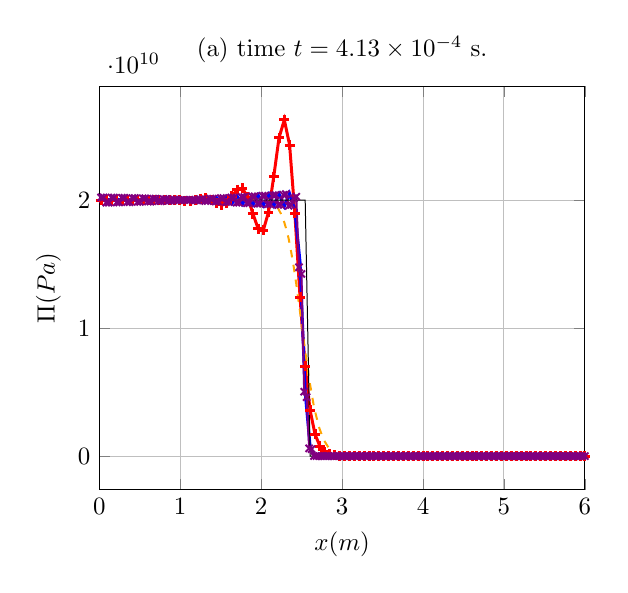
\begin{tikzpicture}[scale=0.9]
\begin{axis}[xlabel=$x (m)$,ylabel=$\Pi (Pa)$,ymajorgrids=true,xmajorgrids=true,legend pos= south west,title={(a) time $t = 4.13\times 10^{-4} $ s.},xmin=0.,xmax=6.]
\addplot[Red,very thick,mark=+,solid] coordinates {(-0.16829522461060809,20007169511.96314) (-0.10369101528636954,19993538918.151154) (-0.03910008978943477,20005752249.60066) (0.025484632606506585,19995780538.002594) (0.09006724602086946,20002982078.92515) (0.1546485608680076,19999277260.36865) (0.2192288029837782,20000480398.382977) (0.2838085169531259,20001789392.278667) (0.3483874448371409,19997301874.53342) (0.41296605184651003,20003008206.491848) (0.4775444471393354,19998613234.28465) (0.5421228879757068,20006614615.093975) (0.6067010779765869,19998205526.77761) (0.6712784021529404,19998711631.528248) (0.7358550513644272,19992106494.35627) (0.8004321132591515,20004770592.319847) (0.8650111473999984,20015779987.73382) (0.9295914037752241,20019625431.191498) (0.9941696099372187,19992929208.032467) (1.0587424231017257,19958300876.966587) (1.123311926789651,19955346446.406406) (1.1878866648233635,20018511640.579197) (1.2524750200748365,20111607980.21578) (1.3170736594252148,20136508388.211338) (1.381663458854595,20010138904.573597) (1.4462219802801475,19778030212.99804) (1.5107477640922773,19635427268.59183) (1.5752752811607438,19797599632.74197) (1.639859880303798,20289327749.506416) (1.70453378203858,20824737676.284462) (1.769262079187512,20916782028.057846) (1.8339384337847504,20225825740.178158) (1.89844144581174,18932646585.446335) (1.9627281077084087,17775081852.48631) (2.026899949421701,17642004813.115726) (2.091185400436795,19055892736.768036) (2.1558364961562164,21827268031.841457) (2.220982442003199,24860462590.307526) (2.286498524038505,26265768115.97021) (2.351967307290947,24295998059.88075) (2.4168137711136564,18956883378.505733) (2.480598163334301,12418144526.81467) (2.543246483139721,7028504053.174823) (2.604999975767945,3579770240.6871147) (2.66618758468537,1694104579.470104) (2.7270670263127124,758612765.168792) (2.7877944080472954,324010645.8165056) (2.848451732493268,132301231.12326287) (2.90907847951511,51629746.688618675) (2.969692513364221,19230481.215198454) (3.0303015063501104,6825460.685392445) (3.0909085945578147,2304741.6481061573) (3.151514997773176,739250.3468689044) (3.212121166898583,224906.37010029136) (3.2727272601131854,64808.36407273517) (3.3333333300016945,17662.648147483887) (3.3939393931074338,4546.039630207806) (3.4545454543493492,1103.2785027445323) (3.5151515151079566,252.0479295361392) (3.5757575757484754,54.104532819766206) (3.6363636363618523,10.890886483248497) (3.69696969696937,2.0511541183492015) (3.7575757575757014,0.36048087591867584) (3.81818181818181,0.05894430243048331) (3.8787878787878776,0.008907404728338756) (3.9393939393939394,0.0011956247957501686) (4.0,0.00011956247957501687) (4.0606060606060606,0.0) (4.121212121212121,0.0) (4.181818181818182,0.0) (4.242424242424242,0.0) (4.303030303030303,0.0) (4.363636363636363,0.0) (4.424242424242425,0.0) (4.484848484848485,0.0) (4.545454545454546,0.0) (4.606060606060606,0.0) (4.666666666666667,0.0) (4.7272727272727275,0.0) (4.787878787878788,0.0) (4.848484848484849,0.0) (4.909090909090909,0.0) (4.96969696969697,0.0) (5.03030303030303,0.0) (5.090909090909091,0.0) (5.151515151515151,0.0) (5.212121212121212,0.0) (5.2727272727272725,0.0) (5.333333333333334,0.0) (5.3939393939393945,0.0) (5.454545454545455,0.0) (5.515151515151516,0.0) (5.575757575757576,0.0) (5.636363636363637,0.0) (5.696969696969697,0.0) (5.757575757575758,0.0) (5.818181818181818,0.0) (5.878787878787879,0.0) (5.9393939393939394,0.0) (6.0,0.0) };
\addplot[Blue,very thick,mark=none,solid] coordinates {(-0.17172662820924992,20126286105.84016) (-0.10660603391933107,19875164406.999718) (-0.04194663943234102,20122512972.128735) (0.022732395165806486,19881553883.263596) (0.08741156754331267,20113695600.0826) (0.15209029604815277,19892923663.406227) (0.21677157984023532,20099953165.28105) (0.2814513737028933,19909115868.450443) (0.3461348221041776,20081472085.12577) (0.4108152742186133,19929906305.25904) (0.4755009353032759,20058503290.3213) (0.5401815288947392,19955007831.504406) (0.6048694507202782,20031358457.677605) (0.6695495822549338,19984074913.32308) (0.7342398618126412,20000405141.87171) (0.7989189035565396,20016709438.584362) (0.8636117080664685,19966060744.260063) (0.9282890378442423,20052467818.751507) (0.9929846146963595,19928785275.12034) (1.0576596352554701,20090869363.82577) (1.1223583072987158,19889072904.409824) (1.1870304528999478,20131405850.072147) (1.2517326020503938,19847442355.372017) (1.3164013359003341,20173552123.78648) (1.3811073800322917,19804426272.137638) (1.4457721874723826,20216777502.470745) (1.5104825561512225,19760559789.583214) (1.575142938446335,20260557805.032604) (1.6398580523466464,19716368448.944717) (1.7045135246263603,20304386827.323605) (1.769233781555915,19672356602.402267) (1.833883876574903,20347788289.080315) (1.8986096450055439,19628995435.82482) (1.96325392193934,20390327196.219734) (2.0279855406761045,19586711664.247425) (2.0926235965346587,20431618631.24346) (2.1573613774425398,19545878506.256725) (2.2219928581092483,20471336442.532116) (2.286737089006318,19506806138.044117) (2.3513616964415003,20505909410.75548) (2.416111827679838,19223361070.797165) (2.4806716443202474,15164119638.328646) (2.544309845123544,4962759374.283854) (2.605921117305293,685282540.4186183) (2.666666666666667,0.0) (2.7272727272727275,0.0) (2.787878787878788,0.0) (2.8484848484848486,0.0) (2.909090909090909,0.0) (2.9696969696969697,0.0) (3.0303030303030303,0.0) (3.090909090909091,0.0) (3.1515151515151514,0.0) (3.2121212121212124,0.0) (3.272727272727273,0.0) (3.3333333333333335,0.0) (3.393939393939394,0.0) (3.4545454545454546,0.0) (3.515151515151515,0.0) (3.5757575757575757,0.0) (3.6363636363636367,0.0) (3.6969696969696972,0.0) (3.757575757575758,0.0) (3.8181818181818183,0.0) (3.878787878787879,0.0) (3.9393939393939394,0.0) (4.0,0.0) (4.0606060606060606,0.0) (4.121212121212121,0.0) (4.181818181818182,0.0) (4.242424242424242,0.0) (4.303030303030303,0.0) (4.363636363636363,0.0) (4.424242424242425,0.0) (4.484848484848485,0.0) (4.545454545454546,0.0) (4.606060606060606,0.0) (4.666666666666667,0.0) (4.7272727272727275,0.0) (4.787878787878788,0.0) (4.848484848484849,0.0) (4.909090909090909,0.0) (4.96969696969697,0.0) (5.03030303030303,0.0) (5.090909090909091,0.0) (5.151515151515151,0.0) (5.212121212121212,0.0) (5.2727272727272725,0.0) (5.333333333333334,0.0) (5.3939393939393945,0.0) (5.454545454545455,0.0) (5.515151515151516,0.0) (5.575757575757576,0.0) (5.636363636363637,0.0) (5.696969696969697,0.0) (5.757575757575758,0.0) (5.818181818181818,0.0) (5.878787878787879,0.0) (5.9393939393939394,0.0) (6.0,0.0) };
\addplot[Orange,thick,mark=none,dashed] coordinates {(-0.17065948135616368,20000043525.826946) (-0.13846405161119207,20000131357.192825) (-0.10615855337338398,20000218494.583206) (-0.07404331926680283,20000306501.181454) (-0.04177810548697509,20000393896.47217) (-0.009673436417956368,20000482254.930782) (0.022584758948793797,20000570082.4036) (0.05468914251045678,20000658972.299118) (0.08694578874198917,20000747409.83799) (0.11905093160937343,20000837015.308666) (0.15130700223550114,20000926246.024586) (0.18341275190367462,20001016757.47824) (0.21566843234413013,20001106971.41286) (0.24777463690422233,20001198587.31625) (0.2800300115792282,20001289983.21988) (0.3121365750418777,20001382911.99803) (0.34439170296599453,20001475699.235306) (0.3764985602426821,20001570161.365646) (0.4087534845749329,20001664562.05299) (0.4408605892235251,20001760792.46614) (0.47311534282934564,20001857043.951477) (0.5052226603149179,20001955294.841774) (0.537477269066949,20002053652.623417) (0.5695847728293589,20002154196.745407) (0.6018392576971193,20002254937.886917) (0.63394692670971,20002358072.38815) (0.6662013049757795,20002461499.472862) (0.69830912223634,20002567550.322327) (0.730563408177844,20002673996.019188) (0.7626713598344566,20002783323.1565) (0.7949255653178342,20002893155.55905) (0.8270336401018328,20003006158.999344) (0.8592877752388308,20003119788.01011) (0.8913959639439372,20003236915.248775) (0.9236500375876889,20003354800.358326) (0.9557583325989031,20003476555.48888) (0.988012352597941,20003599215.36085) (1.0201207475700413,20003726170.38179) (1.0523747209384142,20003854194.74781) (1.0844832106025044,20003987003.679684) (1.1167371437039924,20004121068.23257) (1.1488457237196221,20004260484.92572) (1.1810996224233543,20004401370.18105) (1.2132082892569704,20004548271.07166) (1.2454621590450947,20004696886.54289) (1.2775709098908066,20004852300.090237) (1.309824755958588,20005009715.66264) (1.3419335886911143,20005174860.54694) (1.3741874160526513,20005342346.906036) (1.4062963291967852,20005518680.70837) (1.4385501427858645,20005697758.81623) (1.4706591355042127,20005887046.311424) (1.5029129402719827,20006079555.280518) (1.5350220123805445,20006284041.2585) (1.5672758134024902,20006492358.140556) (1.5993849654540777,20006715414.269215) (1.631638768111729,20006943437.753944) (1.6637480016793325,20007191089.639084) (1.6960018121418028,20007446834.098385) (1.7281111303121328,20007725459.210213) (1.7603649564409494,20008019319.813942) (1.7924743621157493,20008294004.40781) (1.824728211751267,20008585840.13172) (1.8568376886603435,20008554541.09674) (1.8890915456370228,20008462505.522263) (1.9212009637009544,20006730940.889435) (1.9534546670018174,20004485622.310314) (1.9855634459187166,19996264844.062057) (2.0178162660757217,19985866912.241154) (2.049922432994727,19957886954.48237) (2.0821719106575194,19923019878.742535) (2.1142699487559726,19844752482.056076) (2.146509305404184,19748673138.130287) (2.1785861511174294,19561739730.699345) (2.210799592712115,19335939752.423916) (2.24282884289106,18950316261.230713) (2.2749849883928817,18492945635.84119) (2.3069214957996795,17806784492.6505) (2.338967747836579,17010629044.48117) (2.3707479648286887,15966022841.692478) (2.4026123302922753,14785812065.51804) (2.434166526992342,13436743410.941061) (2.4657735751955867,11958066788.981596) (2.497049074903414,10483331170.150602) (2.528347122496258,8916511769.703724) (2.5593295703130683,7540569940.703419) (2.590312212342123,6120676372.669546) (2.6210295241339954,5005409973.170741) (2.651735403923134,3883807857.160711) (2.6822429663855347,3081223065.2520843) (2.712736226853065,2292253118.873356) (2.7430959078472834,1769087143.9346516) (2.773443251962098,1265410542.8025982) (2.803708355333792,951803900.811647) (2.8339646430982732,655843903.0110523) (2.864174119091245,481283905.106187) (2.894378051323549,319756521.6427987) (2.924557159507066,229045727.21750608) (2.954733115412435,146743624.4075898) (2.984896753012443,102624770.99267791) (3.015058747688463,63378554.38021657) (3.0452150104299562,43277421.13854273) (3.075370482653709,25746439.23638048) (3.105523452064602,17166812.660074137) (3.1356760689168683,9830289.851074612) (3.1658276603124804,6400759.483536921) (3.195979105635568,3525021.159262417) (3.226130156857271,2241699.5574820205) (3.2562811517774475,1186278.3528258102) (3.2864320046978017,736934.7477214294) (3.3165828374132054,374402.79637388245) (3.346733622184799,227248.07808513625) (3.3768844002016,110745.8468615504) (3.4070351630577127,65691.86429748994) (3.4371859238094924,30680.492705236302) (3.467336680073573,17790.289802416904) (3.497487435726684,7955.149116569932) (3.5276381901369445,4510.511505733829) (3.55778894438189,1929.1940661950573) (3.587939698304978,1069.8799239515781) (3.6180904521863875,437.2341897356511) (3.6482412059899048,237.23724715030917) (3.6783919597836334,92.53448438029154) (3.7085427135597566,49.13748895850961) (3.73869346733374,18.270581630057357) (3.7688442211040107,9.498103159014207) (3.7989949748738456,3.3623360506506152) (3.82914572864295,1.711835801326188) (3.859296482411972,0.5762313703130271) (3.8894472361808607,0.28742820089864735) (3.9195979899497346,0.09200332803300691) (3.9497487437185868,0.0450750547997889) (3.9798994974874353,0.013749685151127641) (4.01005025125628,0.006635717616413599) (4.040201005025126,0.0019727809129877925) (4.0703517587939695,0.0008967185968126294) (4.100502512562814,0.0003586874387250511) (4.130653266331658,0.00011956247957501691) (4.160804020100502,0.0) (4.190954773869347,0.0) (4.221105527638191,0.0) (4.251256281407035,0.0) (4.281407035175879,0.0) (4.311557788944723,0.0) (4.341708542713568,0.0) (4.371859296482412,-5.9781239787508415e-05) (4.402010050251256,0.0) (4.4321608040201,0.0) (4.4623115577889445,0.0) (4.492462311557789,0.0) (4.522613065326633,0.0) (4.552763819095477,0.0) (4.582914572864321,0.0) (4.613065326633166,0.0) (4.64321608040201,0.0) (4.673366834170854,-5.9781239787508415e-05) (4.703517587939698,0.0) (4.733668341708542,-5.9781239787508415e-05) (4.763819095477387,0.0) (4.793969849246231,0.0) (4.824120603015075,0.0) (4.8542713567839195,0.0) (4.884422110552763,0.0) (4.914572864321608,0.0) (4.944723618090452,0.0) (4.974874371859296,-5.9781239787508415e-05) (5.005025125628141,0.0) (5.035175879396984,-5.9781239787508415e-05) (5.065326633165829,0.0) (5.0954773869346734,0.0) (5.125628140703517,0.0) (5.155778894472362,0.0) (5.185929648241205,0.0) (5.21608040201005,0.0) (5.2462311557788945,0.0) (5.276381909547738,-5.9781239787508415e-05) (5.306532663316583,0.0) (5.3366834170854265,-5.9781239787508415e-05) (5.366834170854271,0.0) (5.396984924623116,0.0) (5.427135678391959,0.0) (5.457286432160804,0.0) (5.487437185929648,0.0) (5.517587939698492,0.0) (5.547738693467337,0.0) (5.57788944723618,-5.9781239787508415e-05) (5.608040201005025,0.0) (5.638190954773869,-5.9781239787508415e-05) (5.668341708542713,0.0) (5.698492462311558,0.0) (5.7286432160804015,0.0) (5.758793969849246,0.0) (5.788944723618091,0.0) (5.819095477386934,0.0) (5.849246231155779,5.978123978750844e-05) (5.879396984924623,-5.9781239787508415e-05) (5.909547738693467,0.0) (5.939698492462312,0.0) (5.969849246231155,0.0) (6.0,0.0) };
\addplot[Purple,thick,mark=x,solid] coordinates {(-0.1708904472675148,19785557608.354362) (-0.141053536291792,19785867406.07991) (-0.10639968665550317,20213101585.682953) (-0.07596722729975139,20213166639.459328) (-0.04207388662674958,19789540452.376034) (-0.011506607675021027,19789557029.70826) (0.022285105176351794,20207044209.230186) (0.052869007707743255,20207022244.274338) (0.08665834628959812,19798347997.174698) (0.1172321822636404,19798342777.723587) (0.151029412846739,20196099111.801785) (0.18158911289003257,20196061786.86517) (0.2154029118177921,19812014870.030228) (0.24594855907990398,19812000299.62603) (0.2797707639479692,20180456497.651028) (0.31030435509337834,20180413575.280464) (0.34414190966292796,19830391975.858875) (0.3746654464197197,19830363703.36432) (0.4085073802039732,20160337163.972836) (0.4390230930475627,20160297191.04402) (0.4728761360608775,19853261920.69269) (0.5033851748227214,19853214144.348965) (0.5372398018663066,20136017953.04032) (0.5677435687389828,20135992244.21921) (0.6016065301582988,19880348866.887726) (0.6321057005127878,19880275931.784782) (0.6659696058844139,20107829473.983624) (0.696465113347797,20107832721.84703) (0.7303345889699686,19911323145.714508) (0.7608267981523694,19911220393.101494) (0.794698155191189,20076150936.708942) (0.8251876402029276,20076201595.577923) (0.8590614435557611,19945806771.791153) (0.8895483774038433,19945671337.662453) (0.9234264348463641,20041403461.894547) (0.9539111397029185,20041524039.151882) (0.9877878427021151,19983380229.063835) (1.0182704154578464,19983211779.396458) (1.0521550389906216,20004041901.242966) (1.0826356465144116,20004259130.529278) (1.1165141722198928,20023590444.9662) (1.146992928994242,20023391823.879498) (1.1808842235337922,19964545222.656155) (1.2113612103069733,19964890116.037624) (1.2452405366181794,20065959588.155254) (1.2757159448575515,20065737455.962234) (1.3096140087494017,19923405655.590446) (1.340087867199397,19923913531.19163) (1.3739668745812406,20109993427.265583) (1.4044394740876944,20109759370.691113) (1.4383442989671855,19881117133.925976) (1.4688156172979114,19881828092.426723) (1.5026930749798657,20155184504.96013) (1.5331634940260768,20154958787.012196) (1.5670749872969294,19838167967.197243) (1.5975444109704615,19839129929.862263) (1.631419066113116,20201034036.189003) (1.6618879405221585,20200860914.39588) (1.695806028986006,19795048344.53005) (1.7262741487880973,19796331467.05578) (1.7601448712991692,20247083731.9241) (1.7906127153916045,20247094549.42775) (1.8245374872621891,19752175452.996067) (1.8550046971339533,19753935406.555477) (1.888870629478351,20292760865.435543) (1.9193376913168196,20293432983.43762) (1.953269542435462,19709654117.014126) (1.9837358641666532,19712407968.009735) (2.0175965864610483,20337138548.75029) (2.048062639992706,20340344997.290543) (2.082002580382462,19666867314.68073) (2.1124672812076257,19672700955.769726) (2.1463232982512577,20378078322.74046) (2.1767870343556104,20391295863.689228) (2.210737854430747,19619814494.093407) (2.241198117559328,19637708700.528072) (2.275052752024238,20408768422.209846) (2.3055096404249302,20461791611.02041) (2.339480401341693,19548900704.7548) (2.3699263513980036,19618213930.10675) (2.4037921787393377,20126713795.32762) (2.4342241255841532,20264753853.55581) (2.468186972434222,14751152292.966133) (2.4985606945703163,14228242465.12349) (2.531508975979028,5032326878.965216) (2.5617596336243342,4603536576.276086) (2.592841768880457,605310239.9535259) (2.623005846412341,539574226.1837834) (2.6532663316582914,0.0005380311580875769) (2.6834170854271355,0.0005380311580875769) (2.7135678391959797,0.0005380311580875769) (2.743718592964824,0.0004782499183000683) (2.7738693467336684,0.0005978123978750856) (2.8040201005025125,0.0005978123978750856) (2.8341708542713566,0.0005380311580875769) (2.8643216080402008,0.0005380311580875769) (2.8944723618090453,0.0005978123978750856) (2.9246231155778895,0.0005978123978750856) (2.9547738693467336,0.0004184686785125597) (2.9849246231155777,0.0003586874387250511) (3.015075376884422,0.0004782499183000683) (3.0452261306532664,0.0004184686785125597) (3.0753768844221105,0.0003586874387250511) (3.1055276381909547,0.0003586874387250511) (3.135678391959799,0.0005380311580875769) (3.165829145728643,0.0005380311580875769) (3.1959798994974875,0.0004184686785125597) (3.2261306532663316,0.0004184686785125597) (3.2562814070351758,0.0004782499183000683) (3.28643216080402,0.0004184686785125597) (3.316582914572864,0.0004782499183000683) (3.3467336683417086,0.0004184686785125597) (3.3768844221105527,0.0004184686785125597) (3.407035175879397,0.0003586874387250511) (3.437185929648241,0.0003586874387250511) (3.467336683417085,0.0003586874387250511) (3.4974874371859297,0.0003586874387250511) (3.527638190954774,0.0003586874387250511) (3.557788944723618,0.0003586874387250511) (3.587939698492462,0.0003586874387250511) (3.618090452261306,0.0003586874387250511) (3.648241206030151,0.0003586874387250511) (3.678391959798995,0.0002989061989375425) (3.708542713567839,0.0002989061989375425) (3.738693467336683,0.0004184686785125597) (3.7688442211055273,0.0004184686785125597) (3.798994974874372,0.0003586874387250511) (3.829145728643216,0.0003586874387250511) (3.85929648241206,0.0001793437193625254) (3.8894472361809043,0.0001793437193625254) (3.9195979899497484,0.0001793437193625254) (3.949748743718593,0.00011956247957501691) (3.979899497487437,0.0003586874387250511) (4.010050251256281,0.0002989061989375425) (4.040201005025126,0.0002989061989375425) (4.0703517587939695,0.0002989061989375425) (4.100502512562814,0.00023912495915003393) (4.130653266331658,0.0003586874387250511) (4.160804020100502,0.0003586874387250511) (4.190954773869347,0.0003586874387250511) (4.221105527638191,0.0003586874387250511) (4.251256281407035,0.0003586874387250511) (4.281407035175879,0.0003586874387250511) (4.311557788944723,0.0003586874387250511) (4.341708542713568,0.0002989061989375425) (4.371859296482412,0.0002989061989375425) (4.402010050251256,0.00023912495915003393) (4.4321608040201,0.00023912495915003393) (4.4623115577889445,0.00023912495915003393) (4.492462311557789,0.00023912495915003393) (4.522613065326633,0.0002989061989375425) (4.552763819095477,0.0002989061989375425) (4.582914572864321,0.0002989061989375425) (4.613065326633166,0.00023912495915003393) (4.64321608040201,0.0003586874387250511) (4.673366834170854,0.0003586874387250511) (4.703517587939698,0.0002989061989375425) (4.733668341708542,0.00023912495915003393) (4.763819095477387,0.0002989061989375425) (4.793969849246231,0.0002989061989375425) (4.824120603015075,0.0002989061989375425) (4.8542713567839195,0.0002989061989375425) (4.884422110552763,0.0003586874387250511) (4.914572864321608,0.0003586874387250511) (4.944723618090452,0.00023912495915003393) (4.974874371859296,0.00023912495915003393) (5.005025125628141,0.0003586874387250511) (5.035175879396984,0.0002989061989375425) (5.065326633165829,0.0002989061989375425) (5.0954773869346734,0.0002989061989375425) (5.125628140703517,0.00023912495915003393) (5.155778894472362,0.0002989061989375425) (5.185929648241205,0.0003586874387250511) (5.21608040201005,0.0003586874387250511) (5.2462311557788945,0.0001793437193625254) (5.276381909547738,0.0001793437193625254) (5.306532663316583,0.0002989061989375425) (5.3366834170854265,0.00023912495915003393) (5.366834170854271,0.00023912495915003393) (5.396984924623116,0.00023912495915003393) (5.427135678391959,0.00023912495915003393) (5.457286432160804,0.00023912495915003393) (5.487437185929648,0.0001793437193625254) (5.517587939698492,0.00011956247957501691) (5.547738693467337,5.978123978750844e-05) (5.57788944723618,5.978123978750844e-05) (5.608040201005025,0.0001793437193625254) (5.638190954773869,0.0001793437193625254) (5.668341708542713,0.00023912495915003393) (5.698492462311558,0.0001793437193625254) (5.7286432160804015,0.00011956247957501691) (5.758793969849246,5.978123978750844e-05) (5.788944723618091,0.00011956247957501691) (5.819095477386934,5.978123978750844e-05) (5.849246231155779,0.0) (5.879396984924623,0.0) (5.909547738693467,0.0) (5.939698492462312,5.978123978750844e-05) (5.969849246231155,-0.0001195624795750168) (6.0,0.0) };
\addplot[black,thin,mark=none,solid] coordinates {(-0.17172662820924992,19999999999.999966) (-0.10660603391933107,19999999999.999966) (-0.04194663943234102,19999999999.999966) (0.022732395165806486,19999999999.999966) (0.08741156754331267,19999999999.999966) (0.15209029604815277,19999999999.999966) (0.21677157984023532,19999999999.999966) (0.2814513737028933,19999999999.999966) (0.3461348221041776,19999999999.999966) (0.4108152742186133,19999999999.999966) (0.4755009353032759,19999999999.999966) (0.5401815288947392,19999999999.999966) (0.6048694507202782,19999999999.999966) (0.6695495822549338,19999999999.999966) (0.7342398618126412,19999999999.999966) (0.7989189035565396,19999999999.999966) (0.8636117080664685,19999999999.999966) (0.9282890378442423,19999999999.999966) (0.9929846146963595,19999999999.999966) (1.0576596352554701,19999999999.999966) (1.1223583072987158,19999999999.999966) (1.1870304528999478,19999999999.999966) (1.2517326020503938,19999999999.999966) (1.3164013359003341,19999999999.999966) (1.3811073800322917,19999999999.999966) (1.4457721874723826,19999999999.999966) (1.5104825561512225,19999999999.999966) (1.575142938446335,19999999999.999966) (1.6398580523466464,19999999999.999966) (1.7045135246263603,19999999999.999966) (1.769233781555915,19999999999.999966) (1.833883876574903,19999999999.999966) (1.8986096450055439,19999999999.999966) (1.96325392193934,19999999999.999966) (2.0279855406761045,19999999999.999966) (2.0926235965346587,19999999999.999966) (2.1573613774425398,19999999999.999966) (2.2219928581092483,19999999999.999966) (2.286737089006318,19999999999.999966) (2.3513616964415003,19999999999.999966) (2.416111827679838,19999999999.999966) (2.4806716443202474,19999999999.999966) (2.544309845123544,19999999999.999966) (2.605921117305293,0.0) (2.666666666666667,0.0) (2.7272727272727275,0.0) (2.787878787878788,0.0) (2.8484848484848486,0.0) (2.909090909090909,0.0) (2.9696969696969697,0.0) (3.0303030303030303,0.0) (3.090909090909091,0.0) (3.1515151515151514,0.0) (3.2121212121212124,0.0) (3.272727272727273,0.0) (3.3333333333333335,0.0) (3.393939393939394,0.0) (3.4545454545454546,0.0) (3.515151515151515,0.0) (3.5757575757575757,0.0) (3.6363636363636367,0.0) (3.6969696969696972,0.0) (3.757575757575758,0.0) (3.8181818181818183,0.0) (3.878787878787879,0.0) (3.9393939393939394,0.0) (4.0,0.0) (4.0606060606060606,0.0) (4.121212121212121,0.0) (4.181818181818182,0.0) (4.242424242424242,0.0) (4.303030303030303,0.0) (4.363636363636363,0.0) (4.424242424242425,0.0) (4.484848484848485,0.0) (4.545454545454546,0.0) (4.606060606060606,0.0) (4.666666666666667,0.0) (4.7272727272727275,0.0) (4.787878787878788,0.0) (4.848484848484849,0.0) (4.909090909090909,0.0) (4.96969696969697,0.0) (5.03030303030303,0.0) (5.090909090909091,0.0) (5.151515151515151,0.0) (5.212121212121212,0.0) (5.2727272727272725,0.0) (5.333333333333334,0.0) (5.3939393939393945,0.0) (5.454545454545455,0.0) (5.515151515151516,0.0) (5.575757575757576,0.0) (5.636363636363637,0.0) (5.696969696969697,0.0) (5.757575757575758,0.0) (5.818181818181818,0.0) (5.878787878787879,0.0) (5.9393939393939394,0.0) (6.0,0.0) };
%\legend{mpm,dgmpm,dgmpm 2ppc,dgmpm 2ppc (RK2),exact}
\end{axis}
\end{tikzpicture}
%%% Local Variables:
%%% mode: latex
%%% TeX-master: "../../mainManuscript"
%%% End:
}
  {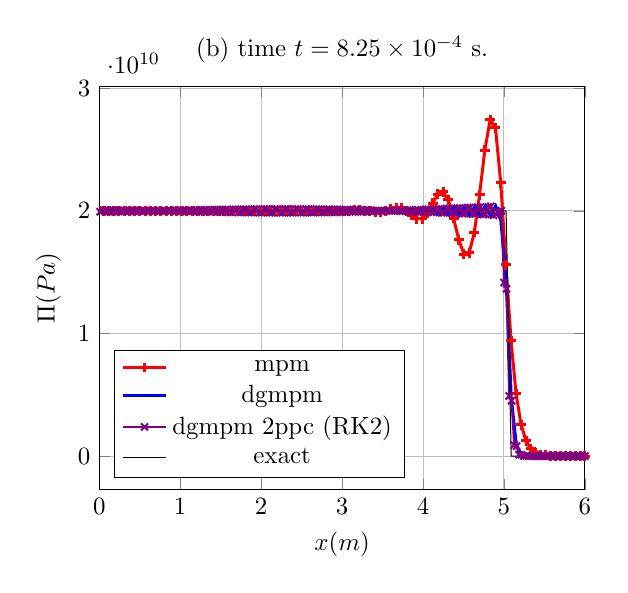
\begin{tikzpicture}[scale=0.9]
\begin{axis}[xlabel=$x (m)$,ylabel=$\Pi (Pa)$,ymajorgrids=true,xmajorgrids=true,legend pos= south west,title={(b) time $t = 8.25\times 10^{-4} $ s.},xmin=0.,xmax=6.]
\addplot[Red,very thick,mark=+,solid] coordinates {(-0.3373970335129395,20002444911.789238) (-0.2727928966297102,19997432693.913857) (-0.20820196231046736,20001959247.078884) (-0.14361740752040095,19997652072.059658) (-0.0790347885190633,20001174478.201954) (-0.014453732919982308,19998113117.396988) (0.050126384917715185,20000219977.304207) (0.1147058039394095,19998668866.378258) (0.17928462960154493,19999250601.410038) (0.24386307172432597,19999169326.347557) (0.30844111377254735,19998402881.7715) (0.3730189157030712,19999501047.64978) (0.43759644654074153,19997762967.548557) (0.50217381047918,19999609942.781967) (0.5667509959420945,19997354773.840668) (0.6313280560675543,19999501477.373802) (0.6959050053014575,19997148374.83382) (0.7604818569685504,19999225474.73323) (0.8250586461934166,19997083680.145477) (0.8896353603808954,19998851023.15548) (0.9542120453300287,19997089910.935226) (1.0187886757648426,19998440828.306694) (1.083365299089184,19997111161.46065) (1.1479418881286723,19998051169.644836) (1.2125184850646817,19997116278.583233) (1.2770950657270574,19997699692.89216) (1.3416716627444705,19997067231.472904) (1.406248258920999,19997388896.74777) (1.4708248806644153,19997000578.277737) (1.535401519422826,19997171020.844025) (1.599978191235337,19996918101.970993) (1.6645548853210443,19996920744.490818) (1.7291316080867047,19996700814.432293) (1.7937083617143608,19996691407.553604) (1.8582851678967984,19996686120.493286) (1.9228620377138623,19996772465.623905) (1.9874389634593603,19996650100.204838) (2.0520159097351134,19996304228.832874) (2.1165928542213344,19995901639.208565) (2.181169830867098,19995922422.124294) (2.245746933014004,19996569013.601753) (2.3103242301117346,19997366737.300365) (2.3749016574282744,19997253707.766594) (2.439479003437918,19995610575.776176) (2.50405608348629,19993366031.355854) (2.5686330012527394,19992897527.09602) (2.633210227393201,19996035016.03268) (2.6977882771955914,20001461417.7394) (2.7623671197745874,20004234447.067886) (2.826945847657703,19999248815.338493) (2.891523147056034,19986954084.876858) (2.9560985175931442,19976226893.658413) (3.020673338478683,19979732556.833313) (3.0852505531422554,20002734650.377262) (3.149832540815079,20033514677.442947) (3.2144183646554727,20045779859.54768) (3.279002790793957,20016543982.692215) (3.343578922732655,19949761640.288918) (3.408143766461,19886271903.166637) (3.472703046370895,19885090545.547707) (3.5372706584700393,19980762153.863453) (3.6018608542803987,20143069670.253544) (3.666476517033703,20272160418.98628) (3.731101311045297,20247014960.951336) (3.7957034722589915,20011400843.260548) (3.8602530814356824,19644164431.403908) (3.924745093767238,19352701051.419342) (3.9892134274545104,19373330976.866657) (4.0537234224180505,19827324507.865147) (4.118341053895788,20606668355.762043) (4.183090744717796,21350802856.75598) (4.247923050028822,21564506017.293846) (4.312715450250743,20887275093.29332) (4.37731903294961,19390073952.106243) (4.441637416097922,17648045449.929543) (4.505695564266106,16477972514.036726) (4.569656065119688,16564993555.823458) (4.633774257438693,18234485218.06143) (4.698311215790016,21316982189.19614) (4.763422276660747,24943663529.441895) (4.829040675663493,27423065710.3382) (4.894809718237837,26786511205.121754) (4.960153433745974,22304704037.851227) (5.024529459659876,15612866271.729282) (5.0877165905602455,9395941456.960642) (5.149868001086729,5080803829.979227) (5.211310703936358,2571948063.5769763) (5.2723407989116975,1251943821.049851) (5.333153160181875,594362859.6955562) (5.393856948062081,276921639.57925117) (5.454508383498881,126868092.89648758) (5.515135140653742,57148823.407327816) (5.575750476779182,25288021.07216049) (5.636360618733436,10978518.189306797) (5.696968440582231,4670443.034755671) (5.757575245750145,1944881.6231991085) (5.818181614449599,792440.4555923982) (5.878787799930788,317032.1081128554) (5.939393910671728,128397.83825474144) (5.9999999928647405,63394.068050559574) };
\addplot[Blue,very thick,mark=none,solid] coordinates {(-0.34300326824190164,19867161670.92257) (-0.27788319029024855,20132353190.445465) (-0.21322278871058642,19869130721.386837) (-0.14854524891661086,20129142425.138195) (-0.08386416618006085,19873652842.561867) (-0.01918775421833607,20123421266.062355) (0.04549613686190245,19880628150.922165) (0.11017305016981589,20115318727.80989) (0.17485949985090674,19889901681.750263) (0.2395368602373047,20105017064.568512) (0.30422552430806427,19901266649.63073) (0.36890325481559005,20092747885.067688) (0.43359370903377453,19914468812.52206) (0.4982717227365738,20078787280.255478) (0.5629635229582883,19929211827.51738) (0.6276417735241854,20063450128.705578) (0.6923344895943412,19945162699.15721) (0.7570129870707453,20047081201.542427) (0.8217062271247281,19961961586.06754) (0.8863850430702915,20030053095.45937) (0.9510784635094146,19979226355.574352) (1.015757722065038,20012756186.25665) (1.0804510262905567,19996560201.361286) (1.1451308857252085,19995591078.27326) (1.2098238162869241,20013559902.98507) (1.2745044463948634,19978961181.23721) (1.339196775641803,20029823630.182865) (1.40387833619713,19963265075.256836) (1.468569859873193,20044958518.655983) (1.533252484114899,19948889080.898514) (1.5979430206134242,20058587899.768158) (1.6626268056632443,19936200167.451828) (1.7273162014193637,20070358058.719982) (1.7920012052713876,19925539314.253044) (1.8566893446755617,20079944419.1636) (1.9213755875853589,19917215422.042995) (1.9860624044406507,20087057076.01931) (2.0507498716789403,19911499852.8977) (2.115435358948472,20091445622.53556) (2.1801240021419153,19908621665.315594) (2.244808217516759,20092903240.062386) (2.3094979529589694,19908763592.066013) (2.3741810192336423,20091270026.991108) (2.4388717231008803,19912058799.92498) (2.503553823894505,20086435560.409016) (2.568245325654722,19918588470.128216) (2.6329266981213357,20078340688.316597) (2.6976187741402335,19928380238.783928) (2.762299700805929,20066978548.729008) (2.826992075723227,19941407541.779408) (2.891672923066381,20052394804.467094) (2.956365346939235,19957589915.641735) (3.0210465161215225,20034687069.70895) (3.0857385707248404,19976794311.40647) (3.150420408966768,20014003488.348423) (3.2151116547381915,19998837479.325516) (3.279794587709358,19990540408.2874) (3.3444845724109693,20023489474.801964) (3.4091690555988876,19964539084.58109) (3.4738573026283968,20050478317.273846) (3.5385438113443364,19936281343.307373) (3.6032298274016155,20079495802.060196) (3.667918848609329,19906084152.544304) (3.732602130509684,20110204420.136734) (3.7972941529817468,19874293081.001152) (3.8619741937006657,20142245283.97256) (3.926669697644514,19841274680.052853) (3.9913459924348733,20175246892.79887) (4.056045440000399,19807407898.849144) (4.120717493458492,20208834504.42018) (4.185421321345374,19773074740.97144) (4.250088655916392,20242639943.665905) (4.314797270727306,19738650272.25273) (4.379459436438253,20276310806.877926) (4.44417321250515,19704493074.44567) (4.508829797148642,20309519959.73904) (4.573549076088961,19670935330.734615) (4.638199714390607,20341974420.673492) (4.702924805180256,19638273500.285717) (4.767569185544008,20373421858.440434) (4.832300363715842,19606757017.834343) (4.896938230755509,20398348853.4957) (4.961674477599282,19194568925.629593) (5.026219132132484,14312041520.443619) (5.089697845458756,4819432981.92643) (5.151288275508455,961012171.3536986) (5.212092547900456,129265691.8128923) (5.272725221999611,10032930.422299773) (5.333333333333334,0.0) (5.3939393939393945,0.0) (5.454545454545455,0.0) (5.515151515151516,0.0) (5.575757575757576,0.0) (5.636363636363637,0.0) (5.696969696969697,0.0) (5.757575757575758,0.0) (5.818181818181818,0.0) (5.878787878787879,0.0) (5.9393939393939394,0.0) (6.0,0.0) };
\addplot[Purple,thick,mark=x,solid] coordinates {(-0.3413421216005564,20084454120.70626) (-0.3115046323967783,20084503231.20538) (-0.2768503231825786,19916185104.896652) (-0.24641699137696205,19916224025.277943) (-0.21252704225382044,20082521029.067745) (-0.18195851890502224,20082494630.53035) (-0.14816447224841806,19919503737.228157) (-0.11757957066435366,19919560593.514977) (-0.08379589265784985,20077952554.12534) (-0.05322085703338879,20077898893.370735) (-0.019419148715127472,19925390458.555717) (0.011141460181846741,19925475541.195904) (0.04494772591031657,20070870972.704773) (0.07549443808768144,20070794153.22469) (0.10932301412763686,19933726420.88046) (0.13985737952332528,19933837024.581604) (0.173685926639547,20061431321.92105) (0.20421035859246994,20061332816.082695) (0.23806014963800134,19944334708.452976) (0.2685764825007371,19944466366.306778) (0.3024195284182063,20049838277.438824) (0.33292927588669197,20049719936.704403) (0.3667927137931127,19956995564.425697) (0.39729694359154255,19957143051.16299) (0.43114948448894214,20036346157.64271) (0.4616491777370185,20036210511.364494) (0.49552220217347964,19971448924.99579) (0.5260180299294327,19971606591.563793) (0.5598772972948788,20021247143.683044) (0.5903698622131245,20021097455.275764) (0.624249900829884,19987369347.34896) (0.654739595219531,19987531478.95478) (0.6886040890282352,20004870125.83432) (0.7190912475113203,20004710463.922737) (0.7529767194177145,20004410302.615177) (0.7834615704641484,20004571380.654194) (0.8173305879064932,19987574487.067276) (0.847813305881258,19987409722.84234) (0.8817031821057704,20022200269.99343) (0.9121839339935235,20022355214.726463) (0.9460571483764127,19969742299.809765) (0.9765360354593392,19969578036.0323) (1.0104294819309994,20040348503.200268) (1.040906682974281,20040492861.37563) (1.0747838335358735,19951770413.041492) (1.105259430932844,19951612839.252544) (1.1391555845596315,20058452407.676346) (1.1696298054671987,20058582471.461685) (1.2035105315252492,19934062461.007298) (1.2339834581168863,19933918134.766502) (1.26788134906568,20076105339.2744) (1.2983532590129288,20076218192.12232) (1.332237072733504,19917020987.71109) (1.3627080375199254,19916896548.399593) (1.3966066343017862,20092904393.807842) (1.4270769595734558,20092997886.904884) (1.4609633199405618,19901039886.204426) (1.4914330391974988,19900941714.78726) (1.5253313681450775,20108457966.61612) (1.5558007815742427,20108530636.852116) (1.58968921499868,19886497320.08024) (1.620158288063799,19886431164.442165) (1.6540555703547062,20122392933.588875) (1.6845245667812516,20122443880.233562) (1.7184147802161702,19873749252.240623) (1.7488835761357309,19873719842.724926) (1.7827793345331566,20134361342.940174) (1.8132481375124534,20134390084.955162) (1.8471400866548187,19863123660.159065) (1.8776086764287256,19863134343.309586) (1.9115027873522425,20144046533.93617) (1.941971308324001,20144052872.731007) (1.9758652132489007,19854915473.262917) (2.00633335571715,19854967893.19228) (2.040226079745077,20151168618.87888) (2.070693985199334,20151152531.999393) (2.104590384682496,19849382232.053566) (2.135057901533144,19849476088.127354) (2.1689496169030114,20155489277.933567) (2.199417036193448,20155450867.5519) (2.2333157795929726,19846740444.56689) (2.263782879164934,19846873351.154137) (2.29767330438176,20156815822.998478) (2.328140263166214,20156755339.15534) (2.3620411522751077,19847162606.42877) (2.392507699460935,19847330075.36992) (2.426397066000551,20155004487.461292) (2.456863380789038,20154922439.98095) (2.4907664359543715,19850774856.538464) (2.5212322666486426,19850970415.948395) (2.555120899476285,20149962895.29097) (2.585586439450331,20149860260.53971) (2.6194915665074547,19857655259.362076) (2.649956589833981,19857870713.761578) (2.6838448104013497,20141651656.730064) (2.7143095156589245,20141530176.422417) (2.7482165060193036,19867832720.558792) (2.7786806902628784,19868058547.559307) (2.8125688393803885,20130084962.0052) (2.8430326926994947,20129947521.903427) (2.8769412584352323,19881286508.15238) (2.907404596472946,19881512377.22646) (2.9412930658856,20115330328.24148) (2.9717560576395274,20115181396.04708) (3.0056658655431305,19897946940.899014) (3.036128344041352,19898162329.4085) (3.070017595121079,20097507428.18806) (3.100479700762355,20097353520.394882) (3.1343903886946634,19917696528.872005) (3.164851976527314,19917891402.385876) (3.1987425343389657,20076785327.117977) (3.2292037151467032,20076635470.893406) (3.2631148843368862,19940372025.717415) (3.29357554543851,19940537544.133724) (3.3274679679788997,20053378728.587624) (3.357928194540636,20053244881.13022) (3.3918393831412645,19965767607.411438) (3.422299107793317,19965896815.490192) (3.456193940921393,20027543050.174908) (3.486653228633958,20027440439.6467) (3.520563880585621,19993639102.67711) (3.5510227208761473,19993727568.79394) (3.5849204556914755,19999568290.3942) (3.615378895931043,19999515651.498085) (3.649288342283673,20023709203.216496) (3.6797464349135187,20023755595.7377) (3.7136474841959903,19969771717.557053) (3.744105255467703,19969791423.13771) (3.7780127218729365,20055673406.51396) (3.8084702852479175,20055680096.82016) (3.8423749893302808,19938489456.48) (3.8728323391771236,19938607645.218704) (3.906736984687898,20089205875.665604) (3.9371942857875872,20089180050.754776) (3.971102948275359,19906067025.556553) (4.001560146502916,19906314216.038258) (4.035461128102997,20123961775.83972) (4.065918424699022,20123919131.594395) (4.099831368443375,19872848196.356743) (4.130288641421362,19873262528.891777) (4.164185191417915,20159573473.009506) (4.194642662567189,20159553030.56887) (4.228560290996899,19839166473.88708) (4.259017750563116,19839808941.31075) (4.292909258187191,20195675341.985744) (4.323366935108609,20195799856.708904) (4.357289795589992,19805336038.508987) (4.387747366655722,19806358551.373158) (4.421633460585793,20231834709.36628) (4.452091150023708,20232554202.447742) (4.48602003137047,19771483196.513275) (4.516477347673006,19773429826.418495) (4.5503580637774,20267126470.97277) (4.58081526693636,20270193617.440983) (4.614751454576072,19736918846.87252) (4.645207821787056,19742059913.02803) (4.679083775444953,20298852761.491997) (4.7095395048223025,20311197166.66586) (4.743485099523246,19697906198.47693) (4.773938201390833,19716155926.428547) (4.807812253028679,20317459432.2131) (4.838261988618075,20366464115.49615) (4.872224665961511,19636335499.984386) (4.9026646932738345,19711246044.137264) (4.936550533899874,19912517877.28153) (4.966975247749498,20015432325.29268) (5.000903022698816,14157492462.311962) (5.031270011791101,13637448020.679394) (5.064107380705877,4900151134.711801) (5.094355634519364,4518545375.67135) (5.125418372928627,896010785.5143551) (5.1555887970834,812792584.0059679) (5.1859044083527275,115327096.28225213) (5.21605773200199,103644640.31290346) (5.246229541628463,7935027.787381989) (5.276380471907977,7067282.007803429) (5.306532663316583,0.0004782499183000683) (5.3366834170854265,0.0005978123978750856) (5.366834170854271,0.0004782499183000683) (5.396984924623116,0.0004782499183000683) (5.427135678391959,0.0004782499183000683) (5.457286432160804,0.0005380311580875769) (5.487437185929648,0.0005380311580875769) (5.517587939698492,0.0004782499183000683) (5.547738693467337,0.0005978123978750856) (5.57788944723618,0.0005978123978750856) (5.608040201005025,0.0005380311580875769) (5.638190954773869,0.0005380311580875769) (5.668341708542713,0.0005380311580875769) (5.698492462311558,0.0005380311580875769) (5.7286432160804015,0.0003586874387250511) (5.758793969849246,0.0002989061989375425) (5.788944723618091,0.0005380311580875769) (5.819095477386934,0.0004782499183000683) (5.849246231155779,0.0004184686785125597) (5.879396984924623,0.0004184686785125597) (5.909547738693467,0.0004782499183000683) (5.939698492462312,0.0004782499183000683) (5.969849246231155,0.0001793437193625254) (6.0,0.00023912495915003393) };
\addplot[black,thin,mark=none,solid] coordinates {(-0.34300326824190164,19999999999.999966) (-0.27788319029024855,19999999999.999966) (-0.21322278871058642,19999999999.999966) (-0.14854524891661086,19999999999.999966) (-0.08386416618006085,19999999999.999966) (-0.01918775421833607,19999999999.999966) (0.04549613686190245,19999999999.999966) (0.11017305016981589,19999999999.999966) (0.17485949985090674,19999999999.999966) (0.2395368602373047,19999999999.999966) (0.30422552430806427,19999999999.999966) (0.36890325481559005,19999999999.999966) (0.43359370903377453,19999999999.999966) (0.4982717227365738,19999999999.999966) (0.5629635229582883,19999999999.999966) (0.6276417735241854,19999999999.999966) (0.6923344895943412,19999999999.999966) (0.7570129870707453,19999999999.999966) (0.8217062271247281,19999999999.999966) (0.8863850430702915,19999999999.999966) (0.9510784635094146,19999999999.999966) (1.015757722065038,19999999999.999966) (1.0804510262905567,19999999999.999966) (1.1451308857252085,19999999999.999966) (1.2098238162869241,19999999999.999966) (1.2745044463948634,19999999999.999966) (1.339196775641803,19999999999.999966) (1.40387833619713,19999999999.999966) (1.468569859873193,19999999999.999966) (1.533252484114899,19999999999.999966) (1.5979430206134242,19999999999.999966) (1.6626268056632443,19999999999.999966) (1.7273162014193637,19999999999.999966) (1.7920012052713876,19999999999.999966) (1.8566893446755617,19999999999.999966) (1.9213755875853589,19999999999.999966) (1.9860624044406507,19999999999.999966) (2.0507498716789403,19999999999.999966) (2.115435358948472,19999999999.999966) (2.1801240021419153,19999999999.999966) (2.244808217516759,19999999999.999966) (2.3094979529589694,19999999999.999966) (2.3741810192336423,19999999999.999966) (2.4388717231008803,19999999999.999966) (2.503553823894505,19999999999.999966) (2.568245325654722,19999999999.999966) (2.6329266981213357,19999999999.999966) (2.6976187741402335,19999999999.999966) (2.762299700805929,19999999999.999966) (2.826992075723227,19999999999.999966) (2.891672923066381,19999999999.999966) (2.956365346939235,19999999999.999966) (3.0210465161215225,19999999999.999966) (3.0857385707248404,19999999999.999966) (3.150420408966768,19999999999.999966) (3.2151116547381915,19999999999.999966) (3.279794587709358,19999999999.999966) (3.3444845724109693,19999999999.999966) (3.4091690555988876,19999999999.999966) (3.4738573026283968,19999999999.999966) (3.5385438113443364,19999999999.999966) (3.6032298274016155,19999999999.999966) (3.667918848609329,19999999999.999966) (3.732602130509684,19999999999.999966) (3.7972941529817468,19999999999.999966) (3.8619741937006657,19999999999.999966) (3.926669697644514,19999999999.999966) (3.9913459924348733,19999999999.999966) (4.056045440000399,19999999999.999966) (4.120717493458492,19999999999.999966) (4.185421321345374,19999999999.999966) (4.250088655916392,19999999999.999966) (4.314797270727306,19999999999.999966) (4.379459436438253,19999999999.999966) (4.44417321250515,19999999999.999966) (4.508829797148642,19999999999.999966) (4.573549076088961,19999999999.999966) (4.638199714390607,19999999999.999966) (4.702924805180256,19999999999.999966) (4.767569185544008,19999999999.999966) (4.832300363715842,19999999999.999966) (4.896938230755509,19999999999.999966) (4.961674477599282,19999999999.999966) (5.026219132132484,19999999999.999966) (5.089697845458756,0.0) (5.151288275508455,0.0) (5.212092547900456,0.0) (5.272725221999611,0.0) (5.333333333333334,0.0) (5.3939393939393945,0.0) (5.454545454545455,0.0) (5.515151515151516,0.0) (5.575757575757576,0.0) (5.636363636363637,0.0) (5.696969696969697,0.0) (5.757575757575758,0.0) (5.818181818181818,0.0) (5.878787878787879,0.0) (5.9393939393939394,0.0) (6.0,0.0) };
\legend{mpm,dgmpm,dgmpm 2ppc (RK2),exact}
\end{axis}
\end{tikzpicture}
%%% Local Variables:
%%% mode: latex
%%% TeX-master: "../../mainManuscript"
%%% End:
}
  \caption{shock stress $50\sigma^y$}
  \label{fig:he_shock}
\end{figure}

\begin{figure}[h!]
  \centering
  {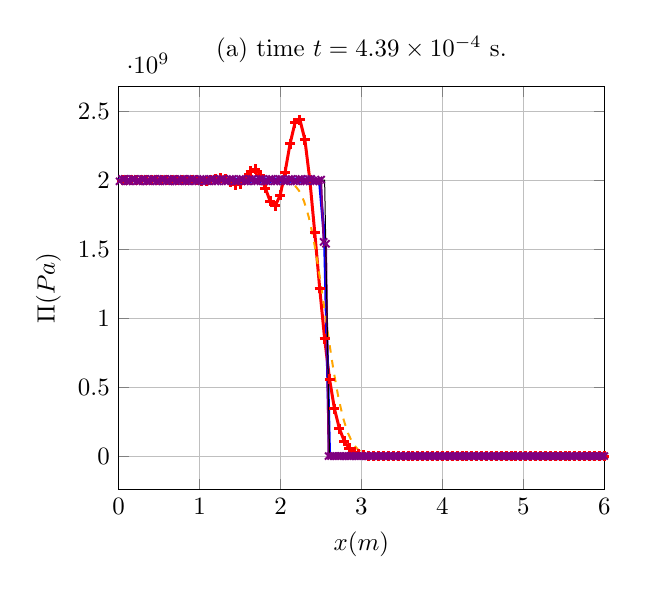
\begin{tikzpicture}[scale=0.9]
\begin{axis}[xlabel=$x (m)$,ylabel=$\Pi (Pa)$,ymajorgrids=true,xmajorgrids=true,legend pos= south west,title={(a) time $t = 4.39\times 10^{-4} $ s.},xmin=0.,xmax=6.]
\addplot[Red,very thick,mark=+,solid] coordinates {(-0.01889090575892736,2000726227.9548469) (0.04215938121847631,1999333692.2170322) (0.10320950300088187,2000564307.210718) (0.1642595721497595,1999551619.5161746) (0.22530959528412595,2000366086.7014122) (0.2863596365377364,1999918681.081198) (0.34740962154368255,1999967513.1983385) (0.4084596019243027,1999982956.3759255) (0.4695095542813397,1999789300.767052) (0.5305595706356425,2000638143.0446692) (0.5916096101001108,2000058185.8142667) (0.6526595840065709,2000089500.8199706) (0.7137094080712463,1998731982.696904) (0.7747591964204517,1999802718.761434) (0.8358092400792819,2001103352.5160503) (0.8968596075653851,2002797653.0377228) (0.9579099107745452,2000545034.2858593) (1.0189595027783396,1996318945.1727874) (1.0800083591701581,1993841183.3513687) (1.1410574970379839,1998917122.885443) (1.2021083083094746,2009171450.4722426) (1.2631608670075336,2014924382.2673836) (1.324213039463032,2005656899.5451016) (1.385261769152474,1983449039.423849) (1.4463061626617941,1966015537.327388) (1.507349635271763,1975043578.4303389) (1.5683984989928055,2015342835.6991093) (1.6294570537824011,2063738687.704247) (1.6905226695860884,2079996363.0337298) (1.7515852284367635,2035769364.3281224) (1.8126325838500514,1940918000.2995517) (1.8736591534269504,1845811486.1301281) (1.9346719362907874,1815039899.0369656) (1.9956894703716108,1889210362.9092839) (2.0567336535453324,2058642788.6612728) (2.117818634233786,2262898814.531011) (2.178942416069636,2414862117.653746) (2.240085148148831,2437155605.434466) (2.301214705448431,2293758990.699916) (2.3622968082809916,2001786574.9585006) (2.4233050712621194,1618923825.3431814) (2.4842269247483553,1216053195.9451652) (2.5450639204752132,851463994.3153192) (2.605827780198291,557925039.8409315) (2.66653493894023,343357124.31856114) (2.7272019233986486,199050644.20604298) (2.7878426090238304,108945510.80319592) (2.8484672666547697,56388618.61462657) (2.9090827809076343,27631268.92148142) (2.9696933946574,12828198.479249047) (3.030301534387653,5645398.76980634) (3.0909084955126,2355626.776140429) (3.15151492615744,932070.1392538762) (3.212121131032279,349709.3400203979) (3.2727272450009446,124397.82639027077) (3.333333324329144,41941.30302034219) (3.3939393911637925,13397.315005244573) (3.4545454537338864,4052.370067713768) (3.515151514926613,1159.9211676619566) (3.5757575756985602,313.92767018390856) (3.6363636363489893,80.26085778895391) (3.6969696969662627,19.36314356717398) (3.7575757575749984,4.402469841671484) (3.8181818181816607,0.9419729953317703) (3.878787878787848,0.1893869676468267) (3.9393939393939337,0.03568940015314253) (3.999999999999999,0.006277030177688385) (4.0606060606060606,0.0010162810763876433) (4.121212121212121,0.00011956247957501687) (4.181818181818182,0.0) (4.242424242424242,0.0) (4.303030303030303,0.0) (4.363636363636363,0.0) (4.424242424242425,0.0) (4.484848484848485,0.0) (4.545454545454546,0.0) (4.606060606060606,0.0) (4.666666666666667,0.0) (4.7272727272727275,0.0) (4.787878787878788,0.0) (4.848484848484849,0.0) (4.909090909090909,0.0) (4.96969696969697,0.0) (5.03030303030303,0.0) (5.090909090909091,0.0) (5.151515151515151,0.0) (5.212121212121212,0.0) (5.2727272727272725,0.0) (5.333333333333334,0.0) (5.3939393939393945,0.0) (5.454545454545455,0.0) (5.515151515151516,0.0) (5.575757575757576,0.0) (5.636363636363637,0.0) (5.696969696969697,0.0) (5.757575757575758,0.0) (5.818181818181818,0.0) (5.878787878787879,0.0) (5.9393939393939394,0.0) (6.0,0.0) };
\addplot[Blue,very thick,mark=none,solid] coordinates {(-0.01905005116856936,2008739016.0347507) (0.04200625800028209,1991261736.4427555) (0.10305754928183601,2008739100.409834) (0.16410893267859902,1991261521.605884) (0.22516022487211998,2008739334.4376273) (0.28621163420310985,1991261157.0218182) (0.3472629006887729,2008739718.3484042) (0.40831433629779745,1991260642.4918854) (0.4693655770844152,2008740252.4789007) (0.5304170389659988,1991259977.710147) (0.591468254064157,2008740937.273132) (0.6525197422102871,1991259162.2632153) (0.713570931632428,2008741773.281487) (0.7746224460325223,1991258195.6316195) (0.8356736097927291,2008742761.1610267) (0.8967251504336042,1991257077.1895308) (0.9577762885477589,2008743901.6730618) (1.0188278554137018,1991255806.2060382) (1.0798789678994447,2008745195.6865165) (1.1409305609721991,1991254381.844086) (1.2019816478489238,2008746644.1731992) (1.2630332671077074,1991252803.1625357) (1.3240843283965613,2008748248.2084675) (1.3851359738180737,1991251069.1156514) (1.4461870095419576,2008750008.9730506) (1.5072386811003957,1991249178.5552225) (1.5682896912839626,2008751927.748467) (1.6293413889510406,1991247130.2292893) (1.690392373620723,2008754005.9189367) (1.7514440973658394,1991244922.7847517) (1.812495056549925,2008756244.9680448) (1.8735468063397946,1991242554.768552) (1.9345977400681083,2008758646.4805305) (1.995649515867116,1991240024.626371) (2.0567004241713285,2008761212.1386473) (2.117752225941453,1991237330.7058423) (2.178803108854988,2008763943.7223768) (2.23985493655583,1991234471.2575831) (2.30090579411386,2008766843.192291) (2.3619576477026816,1991231443.3554277) (2.423008479941872,2008763352.9954166) (2.484060357772498,1983892732.551015) (2.5451094294578325,1563462712.6817071) (2.606060606060606,0.0) (2.666666666666667,0.0) (2.7272727272727275,0.0) (2.787878787878788,0.0) (2.8484848484848486,0.0) (2.909090909090909,0.0) (2.9696969696969697,0.0) (3.0303030303030303,0.0) (3.090909090909091,0.0) (3.1515151515151514,0.0) (3.2121212121212124,0.0) (3.272727272727273,0.0) (3.3333333333333335,0.0) (3.393939393939394,0.0) (3.4545454545454546,0.0) (3.515151515151515,0.0) (3.5757575757575757,0.0) (3.6363636363636367,0.0) (3.6969696969696972,0.0) (3.757575757575758,0.0) (3.8181818181818183,0.0) (3.878787878787879,0.0) (3.9393939393939394,0.0) (4.0,0.0) (4.0606060606060606,0.0) (4.121212121212121,0.0) (4.181818181818182,0.0) (4.242424242424242,0.0) (4.303030303030303,0.0) (4.363636363636363,0.0) (4.424242424242425,0.0) (4.484848484848485,0.0) (4.545454545454546,0.0) (4.606060606060606,0.0) (4.666666666666667,0.0) (4.7272727272727275,0.0) (4.787878787878788,0.0) (4.848484848484849,0.0) (4.909090909090909,0.0) (4.96969696969697,0.0) (5.03030303030303,0.0) (5.090909090909091,0.0) (5.151515151515151,0.0) (5.212121212121212,0.0) (5.2727272727272725,0.0) (5.333333333333334,0.0) (5.3939393939393945,0.0) (5.454545454545455,0.0) (5.515151515151516,0.0) (5.575757575757576,0.0) (5.636363636363637,0.0) (5.696969696969697,0.0) (5.757575757575758,0.0) (5.818181818181818,0.0) (5.878787878787879,0.0) (5.9393939393939394,0.0) (6.0,0.0) };
\addplot[Orange,thick,mark=none,dashed] coordinates {(-0.01889946980668934,2000000476.6320922) (0.011472982262261672,2000001438.4851248) (0.04184684081405173,2000002392.7012472) (0.07221830818119625,2000003356.4999018) (0.1025917130426491,2000004313.5796762) (0.13296300523969845,2000005281.2865465) (0.16333630052391546,2000006243.1661801) (0.19370758569637742,2000007216.7782526) (0.22408085754430615,2000008185.4363225) (0.2544521532603863,2000009167.002689) (0.28482541656310756,2000010144.4770656) (0.3151967209063114,2000011136.1183035) (0.3455699783645009,2000012124.525834) (0.375941289271186,2000013128.4548132) (0.4063145421596361,2000014130.011946) (0.4366858582807102,2000015148.5565734) (0.46705910748905927,2000016165.6025586) (0.49743042788464853,2000017201.230468) (0.5278036740577438,2000018236.2531688) (0.5581749980487619,2000019291.6008966) (0.5885482416749542,2000020347.2658136) (0.6189195687537644,2000021425.1713114) (0.6492928102146956,2000022504.3554904) (0.6796641399908071,2000023607.8955212) (0.7100373795927971,2000024713.7263746) (0.7404087117584984,2000025846.261096) (0.770781949752748,2000026982.1621099) (0.801153284060668,2000028147.3869371) (0.8315265206562344,2000029317.1320484) (0.8618978569046679,2000030519.139193) (0.8922710922772454,2000031726.917393) (0.9226424303005011,2000032970.2716842) (0.9530156645993644,2000034220.765175) (0.9833870042609338,2000035510.5942588) (1.0137602376150086,2000036809.0741432) (1.0441315788021248,2000038151.1810029) (1.0745048113249476,2000039503.6248093) (1.1048761539440453,2000040904.6263094) (1.135249385737295,2000042317.864904) (1.1656207297105001,2000043785.3669105) (1.1959939608663954,2000045267.2687786) (1.2263653061291135,2000046810.0885317) (1.256738536732258,2000048369.7969508) (1.287109883231583,2000049998.2522519) (1.317483113360697,2000051646.4962869) (1.3478544610543197,2000053372.763049) (1.3782276907838837,2000055122.2291121) (1.4085990396392938,2000056960.6600883) (1.4389722690410596,2000058826.1717622) (1.4693436190349667,2000060793.545488) (1.4997168481792058,2000062791.8230162) (1.5300881992973736,2000064911.2737882) (1.560461428254117,2000067066.273204) (1.5908327804937845,2000069397.197215) (1.6212060093376797,2000071787.9900625) (1.6515773627224224,2000074524.9349527) (1.6819505915575537,2000077452.350958) (1.7123219461747121,2000080903.035157) (1.7426951752003998,2000084936.5086977) (1.7730665311339828,2000087540.9977086) (1.803439760589524,2000090978.4911919) (1.8338111168181779,2000077477.0261457) (1.8641843455780502,2000060918.7151618) (1.89455569411346,1999958154.3051436) (1.9249289121352766,1999828194.6022284) (1.9553002169004803,1999383368.9065702) (1.9856733785402865,1998822980.5573165) (2.016044517032017,1997345314.8488786) (2.0464174695217108,1995510656.7783453) (2.076788104100392,1991451764.8388326) (2.1071604354370703,1986509217.5580401) (2.137529784396641,1976980528.1385503) (2.167900564514874,1965628394.4283447) (2.198267080236323,1946149393.6631432) (2.2286345177754954,1923474337.231913) (2.258995557200682,1888386109.4679742) (2.2893566818194317,1848505164.4681375) (2.319708344599485,1792363112.5595503) (2.3500589114299957,1730086099.196376) (2.3803962543095176,1649845080.7546284) (2.410731075812863,1562996199.566734) (2.441048815997596,1460110948.707434) (2.4713625925459266,1351464850.755648) (2.501656185567081,1232676868.5027761) (2.531944653047198,1110279637.2963586) (2.5622113868239693,986331460.2560489) (2.5924723706106327,861678218.7179918) (2.6227120342555033,744346670.210031) (2.652945972784969,629124816.8222382) (2.6831608274884244,527964164.37957025) (2.71337055903147,430909155.97551006) (2.743564662850764,351163528.32019114) (2.7737546123498764,276374743.51695853) (2.8039328190674553,218694935.4413843) (2.8341079548422545,165789527.4489097) (2.8642749709886175,127396775.37849465) (2.8944399082519543,92940066.64930406) (2.9245996662205296,69367708.39847162) (2.9547581309384414,48658784.39870716) (2.9849135418650325,35284991.624521784) (3.015068211540017,23779444.403994165) (3.045221214363269,16758966.548834514) (3.075373824972491,10842273.254041858) (3.1055255924007317,7429200.53377867) (3.1356771679720667,4610317.903746986) (3.165828347947403,3072574.7950721933) (3.195979441069561,1827504.9990729818) (3.2261303619529405,1185127.147576748) (3.2562812464212003,675046.6861063467) (3.2864320612710896,426155.42986476084) (3.3165828619726887,232265.35139310345) (3.346733636544425,142805.4142200062) (3.3768844060203573,74409.37325305404) (3.407035166388237,44577.386497880674) (3.4371859250543553,22185.129789297524) (3.4673366807720183,12956.171896078795) (3.4974874359627095,6152.611330358401) (3.52763819026706,3504.3041958899166) (3.557788944420106,1586.2018885915058) (3.587939698325784,881.5070838911788) (3.618090452191194,379.88885595171956) (3.6482412059925275,206.08344960854643) (3.678391959783931,84.45086513091069) (3.7085427135599374,44.74051898936539) (3.738693467333677,17.410030683202127) (3.7688442211039845,9.011483867110433) (3.798994974873815,3.3249727757824945) (3.8291457286429367,1.6822440876309985) (3.8592964824119647,0.5877093683522783) (3.889447236180857,0.2908357315665427) (3.9195979899497333,0.09612823357834788) (3.9497487437185854,0.04662936703426465) (3.979899497487435,0.014706184987727878) (4.01005025125628,0.0069944050551386675) (4.040201005025126,0.0021521246323503206) (4.0703517587939695,0.001016281076387647) (4.100502512562814,0.0003586874387250511) (4.130653266331658,0.00011956247957501691) (4.160804020100502,5.978123978750844e-05) (4.190954773869347,0.0) (4.221105527638191,0.0) (4.251256281407035,0.0) (4.281407035175879,0.0) (4.311557788944723,0.0) (4.341708542713568,0.0) (4.371859296482412,-5.9781239787508415e-05) (4.402010050251256,0.0) (4.4321608040201,0.0) (4.4623115577889445,0.0) (4.492462311557789,0.0) (4.522613065326633,0.0) (4.552763819095477,0.0) (4.582914572864321,0.0) (4.613065326633166,0.0) (4.64321608040201,0.0) (4.673366834170854,-5.9781239787508415e-05) (4.703517587939698,0.0) (4.733668341708542,0.0) (4.763819095477387,0.0) (4.793969849246231,0.0) (4.824120603015075,0.0) (4.8542713567839195,0.0) (4.884422110552763,0.0) (4.914572864321608,0.0) (4.944723618090452,0.0) (4.974874371859296,0.0) (5.005025125628141,0.0) (5.035175879396984,0.0) (5.065326633165829,0.0) (5.0954773869346734,0.0) (5.125628140703517,0.0) (5.155778894472362,0.0) (5.185929648241205,0.0) (5.21608040201005,0.0) (5.2462311557788945,0.0) (5.276381909547738,-5.9781239787508415e-05) (5.306532663316583,0.0) (5.3366834170854265,-5.9781239787508415e-05) (5.366834170854271,0.0) (5.396984924623116,0.0) (5.427135678391959,0.0) (5.457286432160804,0.0) (5.487437185929648,0.0) (5.517587939698492,0.0) (5.547738693467337,0.0) (5.57788944723618,0.0) (5.608040201005025,5.978123978750844e-05) (5.638190954773869,-5.9781239787508415e-05) (5.668341708542713,0.0) (5.698492462311558,0.0) (5.7286432160804015,0.0) (5.758793969849246,0.0) (5.788944723618091,0.0) (5.819095477386934,-5.9781239787508415e-05) (5.849246231155779,5.978123978750844e-05) (5.879396984924623,0.0) (5.909547738693467,0.0) (5.939698492462312,0.0) (5.969849246231155,0.0) (6.0,0.0) };
\addplot[Purple,thick,mark=x,solid] coordinates {(-0.018953461066473463,1991446661.061328) (0.011194714201811728,1991447340.1765282) (0.04179263124474906,2008553616.6801457) (0.07194754383908661,2008553786.3057418) (0.10253643380986284,1991447493.3310626) (0.13269301032617906,1991447574.3422425) (0.16328078147576108,2008554572.7002) (0.19343774764936655,2008554582.1389053) (0.2240253779425685,1991447859.6478121) (0.25418241511482015,1991447930.5818691) (0.28476989626688765,2008555624.9177055) (0.3149269257596361,2008555623.2558448) (0.3455145674347823,1991448034.9819658) (0.3756715692879528,1991448133.6042144) (0.4062590714943057,2008556842.0924373) (0.4364160416359035,2008556838.9115138) (0.467003771159221,1991448037.4972131) (0.49716070825940945,1991448166.2255507) (0.527748249418257,2008558224.400137) (0.5579051540553267,2008558220.3215702) (0.5884929746851078,1991447868.2226775) (0.6186498466884454,1991448027.2040389) (0.6492374264275679,2008559771.3514504) (0.6793942666629291,2008559766.4251652) (0.7099821771011725,1991447527.543242) (0.7401389854675806,1991447716.7777178) (0.7707266022892127,2008561486.8090549) (0.8008833796675556,2008561481.0619845) (0.8314713783415424,1991447015.2910771) (0.8616281246321296,1991447234.7695084) (0.8922157769826508,2008563372.0888019) (0.922372493064097,2008563365.5949845) (0.9529605783946749,1991446329.7058122) (0.9831172641638408,1991446579.4234667) (1.013704950502113,2008565427.774235) (1.043861606833815,2008565420.8015227) (1.0744497772541894,1991445469.688907) (1.1046064040410184,1991445749.669622) (1.1351941228445261,2008567654.0964527) (1.1653507209569671,2008567647.6765823) (1.195938974915969,1991444434.1637495) (1.2260955442415553,1991444744.559402) (1.2566832940090453,2008570050.2893353) (1.286839835413446,2008570048.467054) (1.3174281713785905,1991443221.7297113) (1.3475846847426682,1991443563.2392223) (1.3781724639980146,2008572611.4914522) (1.4083289501820841,2008572630.206443) (1.4389173666457995,1991441829.765011) (1.469073825519406,1991442205.4102721) (1.4996616328369274,2008575316.3861573) (1.5298180652886002,2008575418.546248) (1.5604065608948054,1991440250.8294203) (1.5905629670328438,1991440673.458793) (1.6211508009003384,2008578078.4761584) (1.651307181902967,2008578512.435198) (1.6818957543055844,1991438457.6398063) (1.7120521100573114,1991438981.576465) (1.7426399679238898,2008580553.9702086) (1.7727962994057174,2008582300.2559524) (1.8033849467032101,1991436340.3404675) (1.833541253464869,1991437194.6760008) (1.8641291340288655,2008581384.4771564) (1.8942854172504617,2008588314.2161562) (1.9248741386090946,1991433444.741186) (1.9550303967770726,1991435593.872973) (1.985618299764926,2008575211.952947) (2.0157745348986764,2008602607.6126542) (2.046363331872024,1991427881.1583545) (2.0765195383045882,1991435378.6636598) (2.1071074672449113,2008540913.448154) (2.1372636502512763,2008649104.02732) (2.167852533779668,1991411780.894133) (2.198008671382919,1991441640.7525687) (2.228596644878877,2008395232.284703) (2.258752754918473,2008822359.8198197) (2.289341773203813,1991352408.047383) (2.3194977696318317,1991475946.8571541) (2.350085866291964,2007809494.577574) (2.3802418153253666,2009495560.7708085) (2.41083116453372,1991111400.0449364) (2.440986728457478,1991626928.107113) (2.471575265426608,1997987384.3139741) (2.5017306963085564,2003928221.7149866) (2.5323193981554217,1552508599.2255695) (2.5624732054671786,1538607374.1694043) (2.5929648241206027,0.000717374877450103) (2.6231155778894473,0.0006575936376625943) (2.6532663316582914,0.0003586874387250511) (2.6834170854271355,0.0003586874387250511) (2.7135678391959797,0.0006575936376625943) (2.743718592964824,0.0006575936376625943) (2.7738693467336684,0.0005978123978750856) (2.8040201005025125,0.0005978123978750856) (2.8341708542713566,0.0005380311580875769) (2.8643216080402008,0.0004782499183000683) (2.8944723618090453,0.00023912495915003393) (2.9246231155778895,0.00023912495915003393) (2.9547738693467336,0.0005380311580875769) (2.9849246231155777,0.0005380311580875769) (3.015075376884422,0.0001793437193625254) (3.0452261306532664,0.0001793437193625254) (3.0753768844221105,0.0005978123978750856) (3.1055276381909547,0.0005380311580875769) (3.135678391959799,0.00023912495915003393) (3.165829145728643,0.00023912495915003393) (3.1959798994974875,0.0004782499183000683) (3.2261306532663316,0.0004184686785125597) (3.2562814070351758,0.0004782499183000683) (3.28643216080402,0.0004782499183000683) (3.316582914572864,5.978123978750844e-05) (3.3467336683417086,0.0) (3.3768844221105527,0.0005978123978750856) (3.407035175879397,0.0005380311580875769) (3.437185929648241,0.00023912495915003393) (3.467336683417085,0.0001793437193625254) (3.4974874371859297,0.0005380311580875769) (3.527638190954774,0.0005380311580875769) (3.557788944723618,0.0005380311580875769) (3.587939698492462,0.0005380311580875769) (3.618090452261306,5.978123978750844e-05) (3.648241206030151,0.00011956247957501691) (3.678391959798995,0.0004782499183000683) (3.708542713567839,0.0004782499183000683) (3.738693467336683,-0.00029890619893754183) (3.7688442211055273,-0.00029890619893754183) (3.798994974874372,0.0005978123978750856) (3.829145728643216,0.0005978123978750856) (3.85929648241206,0.0001793437193625254) (3.8894472361809043,0.00011956247957501691) (3.9195979899497484,0.0001793437193625254) (3.949748743718593,0.00011956247957501691) (3.979899497487437,0.0004184686785125597) (4.010050251256281,0.0004184686785125597) (4.040201005025126,0.0) (4.0703517587939695,-0.0001195624795750168) (4.100502512562814,0.0006575936376625943) (4.130653266331658,0.0005978123978750856) (4.160804020100502,0.0) (4.190954773869347,0.0) (4.221105527638191,0.0002989061989375425) (4.251256281407035,0.00023912495915003393) (4.281407035175879,0.00023912495915003393) (4.311557788944723,0.0001793437193625254) (4.341708542713568,0.0002989061989375425) (4.371859296482412,0.0002989061989375425) (4.402010050251256,-5.9781239787508415e-05) (4.4321608040201,-5.9781239787508415e-05) (4.4623115577889445,0.0006575936376625943) (4.492462311557789,0.0006575936376625943) (4.522613065326633,-0.00032879681883129597) (4.552763819095477,-0.00032879681883129597) (4.582914572864321,0.0008369373570251206) (4.613065326633166,0.0007771561172376117) (4.64321608040201,0.0) (4.673366834170854,-5.9781239787508415e-05) (4.703517587939698,0.0003586874387250511) (4.733668341708542,0.0002989061989375425) (4.763819095477387,-0.00032879681883129597) (4.793969849246231,-0.00029890619893754183) (4.824120603015075,0.0004184686785125597) (4.8542713567839195,0.0003586874387250511) (4.884422110552763,0.0003586874387250511) (4.914572864321608,0.0003586874387250511) (4.944723618090452,0.0004782499183000683) (4.974874371859296,0.0004184686785125597) (5.005025125628141,-0.0001195624795750168) (5.035175879396984,-0.0001195624795750168) (5.065326633165829,0.0005978123978750856) (5.0954773869346734,0.0005978123978750856) (5.125628140703517,0.0) (5.155778894472362,5.978123978750844e-05) (5.185929648241205,0.0006575936376625943) (5.21608040201005,0.0005978123978750856) (5.2462311557788945,-0.00029890619893754183) (5.276381909547738,-0.00029890619893754183) (5.306532663316583,5.978123978750844e-05) (5.3366834170854265,5.978123978750844e-05) (5.366834170854271,0.0002989061989375425) (5.396984924623116,0.00023912495915003393) (5.427135678391959,0.0) (5.457286432160804,-5.9781239787508415e-05) (5.487437185929648,-0.00017934371936252516) (5.517587939698492,-0.00017934371936252516) (5.547738693467337,0.0005978123978750856) (5.57788944723618,0.0005380311580875769) (5.608040201005025,0.0003586874387250511) (5.638190954773869,0.0002989061989375425) (5.668341708542713,-0.00032879681883129597) (5.698492462311558,-0.00032879681883129597) (5.7286432160804015,0.0004782499183000683) (5.758793969849246,0.0004782499183000683) (5.788944723618091,-0.0003885780586188042) (5.819095477386934,-0.0003885780586188042) (5.849246231155779,0.0005978123978750856) (5.879396984924623,0.0005978123978750856) (5.909547738693467,-0.0002391249591500335) (5.939698492462312,-0.0002391249591500335) (5.969849246231155,0.0) (6.0,0.0001793437193625254) };
\addplot[black,thin,mark=none,solid] coordinates {(-0.01905005116856936,2000000000.0000362) (0.04200625800028209,2000000000.0000362) (0.10305754928183601,2000000000.0000362) (0.16410893267859902,2000000000.0000362) (0.22516022487211998,2000000000.0000362) (0.28621163420310985,2000000000.0000362) (0.3472629006887729,2000000000.0000362) (0.40831433629779745,2000000000.0000362) (0.4693655770844152,2000000000.0000362) (0.5304170389659988,2000000000.0000362) (0.591468254064157,2000000000.0000362) (0.6525197422102871,2000000000.0000362) (0.713570931632428,2000000000.0000362) (0.7746224460325223,2000000000.0000362) (0.8356736097927291,2000000000.0000362) (0.8967251504336042,2000000000.0000362) (0.9577762885477589,2000000000.0000362) (1.0188278554137018,2000000000.0000362) (1.0798789678994447,2000000000.0000362) (1.1409305609721991,2000000000.0000362) (1.2019816478489238,2000000000.0000362) (1.2630332671077074,2000000000.0000362) (1.3240843283965613,2000000000.0000362) (1.3851359738180737,2000000000.0000362) (1.4461870095419576,2000000000.0000362) (1.5072386811003957,2000000000.0000362) (1.5682896912839626,2000000000.0000362) (1.6293413889510406,2000000000.0000362) (1.690392373620723,2000000000.0000362) (1.7514440973658394,2000000000.0000362) (1.812495056549925,2000000000.0000362) (1.8735468063397946,2000000000.0000362) (1.9345977400681083,2000000000.0000362) (1.995649515867116,2000000000.0000362) (2.0567004241713285,2000000000.0000362) (2.117752225941453,2000000000.0000362) (2.178803108854988,2000000000.0000362) (2.23985493655583,2000000000.0000362) (2.30090579411386,2000000000.0000362) (2.3619576477026816,2000000000.0000362) (2.423008479941872,2000000000.0000362) (2.484060357772498,2000000000.0000362) (2.5451094294578325,2000000000.0000362) (2.606060606060606,0.0) (2.666666666666667,0.0) (2.7272727272727275,0.0) (2.787878787878788,0.0) (2.8484848484848486,0.0) (2.909090909090909,0.0) (2.9696969696969697,0.0) (3.0303030303030303,0.0) (3.090909090909091,0.0) (3.1515151515151514,0.0) (3.2121212121212124,0.0) (3.272727272727273,0.0) (3.3333333333333335,0.0) (3.393939393939394,0.0) (3.4545454545454546,0.0) (3.515151515151515,0.0) (3.5757575757575757,0.0) (3.6363636363636367,0.0) (3.6969696969696972,0.0) (3.757575757575758,0.0) (3.8181818181818183,0.0) (3.878787878787879,0.0) (3.9393939393939394,0.0) (4.0,0.0) (4.0606060606060606,0.0) (4.121212121212121,0.0) (4.181818181818182,0.0) (4.242424242424242,0.0) (4.303030303030303,0.0) (4.363636363636363,0.0) (4.424242424242425,0.0) (4.484848484848485,0.0) (4.545454545454546,0.0) (4.606060606060606,0.0) (4.666666666666667,0.0) (4.7272727272727275,0.0) (4.787878787878788,0.0) (4.848484848484849,0.0) (4.909090909090909,0.0) (4.96969696969697,0.0) (5.03030303030303,0.0) (5.090909090909091,0.0) (5.151515151515151,0.0) (5.212121212121212,0.0) (5.2727272727272725,0.0) (5.333333333333334,0.0) (5.3939393939393945,0.0) (5.454545454545455,0.0) (5.515151515151516,0.0) (5.575757575757576,0.0) (5.636363636363637,0.0) (5.696969696969697,0.0) (5.757575757575758,0.0) (5.818181818181818,0.0) (5.878787878787879,0.0) (5.9393939393939394,0.0) (6.0,0.0) };
%\legend{mpm,dgmpm,dgmpm 2ppc,dgmpm 2ppc (RK2),exact}
\end{axis}
\end{tikzpicture}
%%% Local Variables:
%%% mode: latex
%%% TeX-master: "../../mainManuscript"
%%% End:
}
  {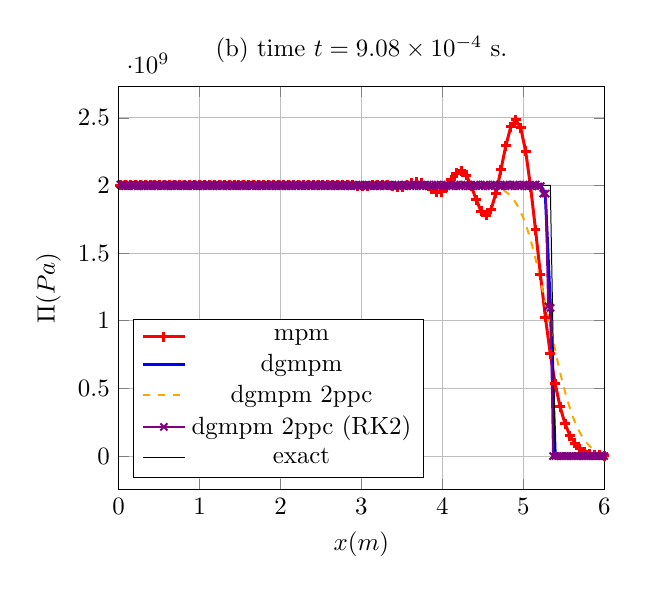
\begin{tikzpicture}[scale=0.9]
\begin{axis}[xlabel=$x (m)$,ylabel=$\Pi (Pa)$,ymajorgrids=true,xmajorgrids=true,legend pos= south west,title={(b) time $t = 9.08\times 10^{-4} $ s.},xmin=0.,xmax=6.]
\addplot[Red,very thick,mark=+,solid] coordinates {(-0.03923052052922343,2000240481.1233327) (0.021819761015892163,1999769738.8663158) (0.0828698927161351,2000218983.1347811) (0.1439199523557292,1999809950.54204) (0.20496998238621425,2000170838.6984289) (0.266019997207666,1999872129.80287) (0.32706999231126516,2000106436.8640933) (0.38811998365041567,1999944280.2454906) (0.449169959029736,2000038581.9512253) (0.510219934372632,2000013690.4345057) (0.5712698969291694,1999979089.5826085) (0.6323198600631447,2000070050.8467832) (0.6933698136476303,1999936253.3022394) (0.7544197669696648,2000107588.3199086) (0.8154697138768967,1999913395.649439) (0.876519659147888,2000125156.8768682) (0.9375696007168677,1999909211.6999958) (0.9986195394150338,2000126157.9927893) (1.059669476515721,1999919755.674749) (1.1207194099155477,2000115626.1187456) (1.1817693429480685,1999938103.4741611) (1.2428192719189772,2000098747.9520392) (1.3038692012782542,1999960657.9597352) (1.3649191269853391,2000083196.644746) (1.4259690532702223,1999982772.5176466) (1.4870189759372838,2000065998.3151865) (1.548068898510965,1999996968.6891499) (1.6091188183068375,2000054865.2647946) (1.670168739008601,2000018826.7281826) (1.731218658453022,2000056284.8743527) (1.7922685772512423,2000025238.8196642) (1.8533184921045645,2000031968.1138716) (1.9143684047609901,2000016400.7497857) (1.975418318053308,2000048568.7818315) (2.0364682364589175,2000073517.7988975) (2.097518157338219,2000081126.454338) (2.158568072062211,2000026752.5138342) (2.2196179727824346,1999962203.1821125) (2.2806678657928665,1999965067.139214) (2.341717771696925,2000088677.3296564) (2.4027677072086253,2000244140.0735695) (2.463817659277123,2000248079.915646) (2.5248675831316487,1999993716.8853536) (2.585917440063807,1999643305.288324) (2.646967250875889,1999579001.41102) (2.7080171068001158,2000062944.273291) (2.7690671011838006,2000852362.1540391) (2.830117219896753,2001206846.0073657) (2.8911672958158867,2000467231.4954524) (2.952217111542271,1998832793.1242473) (3.013266610958221,1997579685.768277) (3.0743160452078344,1998242489.666675) (3.1353658703158658,2001160849.0509126) (3.196416388566518,2004588933.5455565) (3.257467375954363,2005458038.2563794) (3.3185180466647264,2001697102.190524) (3.3795675234732467,1994541487.4730227) (3.440615585708569,1988762645.3894498) (3.5016631438647106,1989935602.9797668) (3.5627119421792885,2000111386.41128) (3.623763471464838,2014923977.0724418) (3.6848176974855837,2024790001.3711026) (3.7458725195458533,2020382377.2601633) (3.8069245712514714,1999447389.7073095) (3.8679711628702065,1970442647.6100123) (3.929012327573847,1949825797.016439) (3.9900516480144432,1953585186.3226125) (4.051095073761827,1987368815.1052973) (4.112148038363928,2040849436.9858987) (4.173212220481733,2090050737.5576959) (4.234283670427938,2107411656.1073942) (4.295353507700337,2075285788.362349) (4.356411206000879,1996293178.97995) (4.417449188621994,1894985293.978191) (4.478466731235185,1809589469.956608) (4.539471418899192,1777676873.8302789) (4.60047747902865,1822118201.7227845) (4.661501591798265,1942507354.7681544) (4.722557637422781,2114144751.4232287) (4.783652041946421,2294062789.964336) (4.844781069302256,2432159789.043516) (4.9059308043019065,2484574935.165112) (4.96707981812872,2425532064.97198) (5.028203724005535,2253708085.122853) (5.0892802390172465,1990804259.1885338) (5.150293249469595,1673238957.9983215) (5.211234847071616,1340859784.348242) (5.272105144435457,1027275994.3558226) (5.332910451399713,754633075.0224329) (5.393660750710443,533012801.80897325) (5.454367310619323,362876107.24577975) (5.515040918237955,238609504.42548501) (5.5756908552374504,151790024.9898157) (5.636324503231241,93541463.05793001) (5.696947375682255,55910425.71914032) (5.7575633798909625,32464567.359246336) (5.818175162719966,18385124.7089494) (5.878784450683184,10291867.039909834) (5.939392341636735,5971073.523642217) (5.999999537141593,4112438.7996382113) };
\addplot[Blue,very thick,mark=none,solid] coordinates {(-0.03942160478635286,2006060116.9510684) (0.021634703667567715,1993940137.594559) (0.08268599644388969,2006060373.9301388) (0.14373737764912256,1993939604.21122) (0.20478867280919388,2006061026.086628) (0.26584007847159263,1993938675.6310308) (0.32689134939619946,2006062073.480748) (0.38794277985880155,1993937351.85318) (0.4489940265576721,2006063516.189758) (0.5100454818139241,1993935632.8617878) (0.571096704298863,2006065354.3060572) (0.6321481843393669,1993933518.6248724) (0.6931993826243398,2006067587.9363937) (0.7542508874368217,1993931009.095019) (0.8153020615377354,2006070217.2044432) (0.876353591107017,1993928104.2093496) (0.9374047410418783,2006073242.2485344) (0.9984562953499471,1993924803.890371) (1.0595074211388207,2006076663.222377) (1.1205590001648187,1993921108.0437915) (1.1816101018298202,2006080480.2947278) (1.2426617055500626,1993917016.5617368) (1.3037127831153568,2006084693.6486328) (1.3647644115033453,1993912529.3202007) (1.4258154649951433,2006089303.4830647) (1.48686711802158,1993907646.1796832) (1.5479181474681376,2006094310.0113149) (1.6089698251009463,1993902366.9880114) (1.6700208305325863,2006099713.4611773) (1.7310725327370886,1993896691.5758796) (1.792123514186276,2006105514.0745523) (1.853175240924819,1993890619.7603688) (1.9142261984258384,2006111712.10775) (1.9752779496581556,1993884151.3441877) (2.0363288832474176,2006118307.831492) (2.097380658930556,1993877286.1154313) (2.1584315686465,2006125301.5292413) (2.21948336873485,1993870023.8487618) (2.28053425461794,2006132693.498629) (2.3415860790632617,1993862364.3047736) (2.4026369411559783,2006140484.0500283) (2.463688789907431,1993854307.2305677) (2.524739628254281,2006148673.5077674) (2.5857915012584574,1993845852.3584197) (2.6468423159059484,2006157262.2078867) (2.7078942131069095,1993836999.410417) (2.7689450041035615,2006166250.4990761) (2.8299969254428645,1993827748.093002) (2.891047692839202,2006175638.7426183) (2.9520996382559384,1993818098.1014004) (3.0131503821044743,2006185427.3114746) (3.074202351535314,1993808049.1178594) (3.13525307189056,2006195616.5906525) (3.196305065269774,1993797600.8137424) (3.2573557621882188,2006206206.9747465) (3.318407779447733,1993786752.8469522) (3.379458452987844,2006217198.8708515) (3.4405104940572713,1993775504.865476) (3.5015611442794836,2006228592.6960747) (3.562613209086164,1993763856.5055692) (3.6236638360528746,2006240388.8765044) (3.684715924521922,1993751807.3932695) (3.745766528297479,2006252587.8494554) (3.806818640351814,1993739357.1445801) (3.8678692210025045,2006265190.0607684) (3.9289213565629106,1993726505.364711) (3.9899719141569547,2006278195.9650536) (4.051024073142108,1993713251.6505055) (4.112074607749643,2006291606.0248404) (4.173126790076167,1993699595.5889838) (4.234177301769245,2006305420.7115803) (4.295229507351752,1993685536.758891) (4.356279996204306,2006319640.5037947) (4.4173322249554365,1993671074.7315753) (4.478382691043292,2006334265.886256) (4.539434942873767,1993656209.068866) (4.600485386274613,2006349297.3502934) (4.661537661093276,1993640939.3284109) (4.72258808188665,2006364735.3943052) (4.783640379600513,1993625265.0586715) (4.844690777867787,2006380580.5203645) (4.905743098382081,1993609185.8030493) (4.966793474206442,2006396833.2363412) (5.027845817424658,1993592701.0995812) (5.088896170891094,2006413494.1091921) (5.149948536715043,1993575783.3857787) (5.2109988679040695,2006188385.7824419) (5.272051199443885,1928173675.83211) (5.333086626305186,1114893331.7484362) (5.3939393939393945,0.0) (5.454545454545455,0.0) (5.515151515151516,0.0) (5.575757575757576,0.0) (5.636363636363637,0.0) (5.696969696969697,0.0) (5.757575757575758,0.0) (5.818181818181818,0.0) (5.878787878787879,0.0) (5.9393939393939394,0.0) (6.0,0.0) };
\addplot[Orange,thick,mark=none,dashed] coordinates {(-0.03917078051451722,2000000162.3641174) (-0.008798328514825843,2000000488.4820786) (0.02157552989991438,2000000813.2866108) (0.051946997059085696,2000001139.558676) (0.08232040164605842,2000001464.592103) (0.11269169349583695,2000001791.172434) (0.14306498836737944,2000002116.5878267) (0.17343627305229423,2000002443.631678) (0.20380954434819964,2000002769.5829566) (0.23418083943507145,2000003097.2461593) (0.26455410204486396,2000003423.8882744) (0.29492540561539754,2000003752.3279023) (0.32529866223778026,2000004079.8172007) (0.3556699722260966,2000004409.1920872) (0.38604322413345515,2000004737.6865525) (0.4164145391877686,2000005068.1573205) (0.4467877872668746,2000005397.8171813) (0.4771591064441345,2000005729.5467284) (0.5075323513364826,2000006060.534245) (0.5379036739539097,2000006393.6881065) (0.5682769161439751,2000006726.1685727) (0.5986482416896831,2000007060.9151359) (0.6290214815546709,2000007395.0570292) (0.6593928096333185,2000007731.5681388) (0.6897660474744984,2000008067.5430918) (0.7201373777728655,2000008405.9942615) (0.7505106138357185,2000008743.9778793) (0.7808819461002032,2000009084.5488696) (0.8112551805873307,2000009424.7210948) (0.8416265146091947,2000009767.5960035) (0.8719997476890129,2000010110.141691) (0.9023710832946423,2000010455.5098622) (0.9327443151082355,2000010800.6187513) (0.9631156521521939,2000011148.6750796) (0.9934888828192661,2000011496.5425496) (1.023860221178728,2000011847.4878132) (1.0542334508024265,2000012198.3157957) (1.0846047903724751,2000012552.357385) (1.114978019042759,2000012906.3543007) (1.1453493597326887,2000013263.7067938) (1.1757225875285224,2000013621.0883734) (1.2060939292591928,2000013981.9742343) (1.2364671562501526,2000014342.964246) (1.2668384989521082,2000014707.6141872) (1.2972117251998054,2000015072.4452546) (1.327583068811835,2000015441.0991797) (1.3579562943711885,2000015810.0127223) (1.3883276388390875,2000016182.9205422) (1.4187008637593828,2000016556.168837) (1.4490722090348958,2000016933.5912306) (1.479445433360601,2000017311.4369278) (1.5098167794005606,2000017693.6460981) (1.540190003171984,2000018076.364191) (1.5705613499376172,2000018463.64511) (1.600934573191448,2000018851.5232396) (1.6313059206478067,2000019244.1745574) (1.6616791434175868,2000019637.514589) (1.6920504915330754,2000020035.8497267) (1.7224237138495884,2000020434.9682348) (1.752795062595561,2000020839.3167174) (1.783168284487177,2000021244.54714) (1.8135396338376049,2000021655.256114) (1.8439128553305595,2000022066.9496617) (1.874284205261732,2000022484.3848658) (1.9046574263803855,2000022902.912099) (1.9350287768706722,2000023327.4603496) (1.9654019976377166,2000023753.2127259) (1.995773348667354,2000024185.283102) (2.026146569104,2000024618.6753104) (2.056517920654903,2000025058.701214) (2.0868911407810526,2000025500.1727536) (2.117262492836659,2000025948.6143074) (2.1476357126710357,2000026398.631942) (2.1780070652161907,2000026855.9786568) (2.2083802847764655,2000027315.038813) (2.2387516377972774,2000027781.8113482) (2.2691248571002074,2000028250.4430869) (2.299496210583961,2000028727.197738) (2.3298694296454614,2000029205.9659374) (2.360240783580518,2000029693.2966387) (2.390614002415777,2000030182.80506) (2.420985356791518,2000030681.3481157) (2.4513585754150644,2000031182.2437081) (2.4817299302217974,2000031692.6813707) (2.512103148647591,2000032205.6581848) (2.5424745038765173,2000032728.723872) (2.5728477221179986,2000033254.5284579) (2.6032190777611506,2000033791.011848) (2.633592295831322,2000034330.4484112) (2.6639636518815353,2000034881.2016294) (2.6943368697930166,2000035435.1385217) (2.724708226243874,2000036001.0829961) (2.7550814440089666,2000036570.4594786) (2.785452800854792,2000037152.5936723) (2.8158260184855197,2000037738.4283779) (2.8461973757213492,2000038337.8370101) (2.8765705932295256,2000038941.2369497) (2.9069419508510856,2000039559.100701) (2.9373151682483614,2000040181.272001) (2.9676865262520598,2000040818.8798575) (2.998059743549965,2000041461.1396496) (3.0284311019329078,2000042119.902398) (3.058804319142925,2000042783.693527) (3.0891756779028725,2000043465.1593158) (3.119548895036467,2000044152.0662634) (3.149920254171894,2000044857.9392831) (3.1802934712405904,2000045569.707488) (3.210664830750652,2000046301.8697186) (3.241038047766071,2000047040.4279282) (3.271409407650652,2000047800.9644024) (3.3017826246245887,2000048568.4518778) (3.332153984884333,2000049359.6807387) (3.3625272018288044,2000050158.4777672) (3.3928985624651316,2000050982.9869034) (3.423271779392468,2000051815.7531936) (3.4536431404076353,2000052676.442854) (3.4840163573305416,2000053546.1624532) (3.514387718727702,2000054446.298109) (3.544760935659359,2000055356.334058) (3.5751322974426225,2000056299.6104584) (3.6055055143967873,2000057253.7731807) (3.6358768765713187,2000058244.4001842) (3.666250093562429,2000059247.0382943) (3.696621456134557,2000060289.8701007) (3.726994673177886,2000061346.020349) (3.7573660361552457,2000062446.766893) (3.7877392532670706,2000063562.4175744) (3.8181106166588106,2000064727.8445463) (3.8484838338566654,2000065910.2265694) (3.878855197673629,2000067147.2274063) (3.9092284149765657,2000068403.7688186) (3.9395997792308908,2000069711.460432) (3.969972996658988,2000071040.1196663) (4.000344361360155,2000072372.298481) (4.030717578929703,2000073715.0698273) (4.061088944065783,2000074840.6027808) (4.091462161766081,2000075910.8957367) (4.1218335272342905,2000075973.490028) (4.152206744942054,2000075715.9219925) (4.182578110329392,2000072017.5705454) (4.212951327539943,2000067131.4477975) (4.243322691511244,2000052136.1276474) (4.273695906596111,2000033486.8974528) (4.304067265361103,1999988181.887949) (4.334440473729889,1999932969.7635126) (4.364811817560196,1999813571.3437288) (4.395185007538841,1999669911.3315077) (4.425556313547598,1999383776.7298186) (4.4559294579562065,1999043281.0910368) (4.4863006763964615,1998409529.043498) (4.516673716815124,1997663436.0152357) (4.547044747257358,1996355344.6753125) (4.577417567129801,1994831959.2009664) (4.607788220571398,1992302969.86891) (4.638160603215137,1989389898.2979999) (4.668530547222314,1984793672.304229) (4.6989021163023,1979557932.6497817) (4.729270803483105,1971684482.5656424) (4.759640947321604,1962815620.4939368) (4.790007533184552,1950076775.4725223) (4.820375320667521,1935888669.9438126) (4.85073858472269,1916391308.5814097) (4.881102688721596,1894921195.4833472) (4.911460980662173,1866658935.7383642) (4.9418196326105,1835890533.9691072) (4.972170870339898,1797058943.0501766) (5.002521873397632,1755266449.2887096) (5.032863617674702,1704664533.4364638) (5.063204441934459,1650828834.6829815) (5.093534060621755,1588261707.5287433) (5.1238620296206765,1522463019.1566145) (5.154176943201123,1449027996.623211) (5.184489497747455,1372692658.5953019) (5.214787471910191,1290836359.622366) (5.245082470974608,1206731514.3493056) (5.275361900847146,1120019487.5397825) (5.305637899924566,1031954086.5330459) (5.335898023815224,944583266.5800234) (5.366154468378211,856867538.3261541) (5.396395461927203,773038830.7005187) (5.426632751210188,689836677.529801) (5.456855682417766,613149742.0165061) (5.487075091582609,537890878.0345305) (5.517281752431922,470906162.1372124) (5.547485236836296,405894014.3081077) (5.5776778950914725,349940731.67696774) (5.607867825779997,296217313.58628106) (5.638048952254623,251444398.38318378) (5.668227839460561,208891324.5259999) (5.698399860557165,174495130.29764324) (5.728570112675359,142092567.12201983) (5.7587352207461455,116627311.01028177) (5.788898966675067,92773016.07205984) (5.8190589997605136,74455848.39195786) (5.8492179810898115,57259214.528929405) (5.879374365625287,44208394.22829007) (5.90952988824298,31705107.093837854) (5.93968362704645,22082669.924264487) (5.9698365523275365,12349931.960094882) (5.999988236235052,4409369.507638947) };
\addplot[Purple,thick,mark=x,solid] coordinates {(-0.03922301604942032,1994135003.8143709) (-0.009074837831142603,1994135327.5382233) (0.021523075320129238,2005865460.1935375) (0.051677994339231634,2005865540.6397502) (0.0822668758008341,1994135396.4583592) (0.11242345978014313,1994135442.2756677) (0.14301122575351569,2005866580.2736385) (0.17316819949872822,2005866583.7764273) (0.20375581897468137,1994135235.3830903) (0.23391286390200003,1994135281.970573) (0.26450034123994165,2005868078.4857993) (0.29465737837952566,2005868076.052185) (0.3252450076005887,1994134650.7495997) (0.3554020172291876,1994134716.185983) (0.38598951715446034,2005869987.9532342) (0.41614649494956335,2005869984.196581) (0.44673421042392686,1994133650.8641272) (0.4768911553029312,1994133736.3200936) (0.5074786957261858,2005872310.7698147) (0.5376356080195605,2005872305.9982176) (0.5682234130066373,1994132236.1149685) (0.5983802927916309,1994132341.6644566) (0.6289678733432371,2005875047.0253694) (0.6591247212380037,2005875041.269826) (0.6897126144378939,1994130406.364448) (0.7198694305893111,1994130532.0101562) (0.750457049772885,2005878196.6928372) (0.7806138348143057,2005878189.968179) (0.8112018146518958,1994128161.431707) (0.8413585687314308,1994128307.172391) (0.8719462249947207,2005881759.749104) (0.9021029487435118,2005881752.0713456) (0.93269101363723,1994125501.1181188) (0.9628477071998897,1994125666.9514115) (0.9934353990033135,2005885736.186498) (1.02359206300724,2005885727.5732303) (1.0541802113876557,1994122425.2141414) (1.0843368459731915,1994122611.1380703) (1.1149245717959766,2005890126.0066001) (1.145081177586202,2005890116.477569) (1.1756694078991365,1994118933.5003204) (1.20582598502954,1994119139.512731) (1.2364137433721918,2005894929.2238271) (1.2665702924608768,2005894918.8010514) (1.297158603170002,1994115025.7430112) (1.3273151243468142,1994115251.8416276) (1.3579029137342808,2005900145.8680048) (1.388059407611098,2005900134.575021) (1.418647797202381,1994110701.6970189) (1.4488042639020475,1994110947.8799276) (1.4793920829061942,2005905775.9789429) (1.5095485230651517,2005905763.8418655) (1.5401369901663489,1994105961.1079912) (1.5702934041634364,1994106227.373129) (1.6008812512548274,2005911819.6044917) (1.6310376400017392,2005911806.6511338) (1.6616261822127902,1994100803.712939) (1.691782545932699,1994101090.0580282) (1.7223704184836093,2005918276.7966) (1.7525267578346984,2005918263.0567758) (1.7831153730505365,1994095229.246782) (1.81327168818946,1994095535.669637) (1.84385958458336,2005925147.5690346) (1.8740158761491597,2005925133.0745907) (1.9046045627390318,1994089237.483962) (1.9347608308802464,1994089563.9823666) (1.9653487495801851,2005932431.753553) (1.9955049949309274,2005932416.5382469) (2.0260937512936668,1994082828.3726115) (2.0562499739975535,1994083174.944045) (2.0868379134903403,2005940128.4045188) (2.116994114177042,2005940112.50405) (2.1475829387283234,1994076002.632435) (2.1777391175363148,1994076369.2744386) (2.2083270763308156,2005948238.0659459) (2.2384832338849914,2005948221.518105) (2.269072125058446,1994068763.590026) (2.29922826149173,1994069150.2999275) (2.3298162381208245,2005956761.6554585) (2.359972354052955,2005956744.5004637) (2.3905613103018015,1994061110.0614216) (2.420717405859752,1994061516.8370643) (2.45130539888087,2005965699.5618157) (2.481461474678868,2005965681.8411288) (2.5120504944773168,1994053037.4510324) (2.5422065506359943,1994053464.2903204) (2.5727945586318346,2005975052.6724114) (2.6029505957595642,2005975034.4297986) (2.633539677604385,1994044544.567231) (2.663695695815098,1994044991.4683108) (2.694283717395741,2005984821.1414673) (2.7244397172916366,2005984802.422394) (2.755028859703366,1994035631.0282984) (2.7851848413913207,1994036097.989225) (2.8157728751957185,2005995004.9483852) (2.8459288392714592,2005994985.8002572) (2.8765180407956676,1994026296.6488297) (2.906673987358701,1994026783.6678703) (2.937262032055926,2006005604.0494888) (2.9674179616952228,2006005584.521593) (2.998007220903698,1994016541.2667468) (3.028163133711092,1994017048.3420172) (3.0587511880014775,2006016618.410417) (3.0889070845589246,2006016598.5542543) (3.119496400050816,1994006364.723129) (3.1496522804421927,1994006891.8527138) (3.180240343058371,2006028048.018772) (3.2103962078583868,2006028027.8874202) (3.240985578261241,1993995766.8365867) (3.271141427545555,1993996314.0189655) (3.3017294972534104,2006039892.8819644) (3.331885331589273,2006039872.530837) (3.3624747555599876,1993984747.4102676) (3.3926305750146017,1993985314.6443734) (3.42321865061413,2006052153.0306427) (3.453374455747092,2006052132.518732) (3.48396393197279,1993973306.2256682) (3.5141197228426364,1993973893.512831) (3.544707803168714,2006064828.5125036) (3.574863580327216,2006064807.9070828) (3.6054531075260225,1993961443.0478823) (3.635608871022857,1993962050.3986511) (3.666196954945923,2006077919.3870173) (3.6963527053248892,2006077898.7828076) (3.7269422822466223,1993949157.6075246) (3.7570980195483576,1993949785.0704486) (3.7876861059750215,2006091425.6997945) (3.8178418307352264,2006091405.2948232) (3.848431456162036,1993936449.554937) (3.878587168412147,1993937097.334268) (3.909175256285717,2006105347.3760405) (3.939330956553215,2006105327.7684526) (3.9699206293001703,1993923318.2738523) (4.000076317607094,1993923987.2069037) (4.030664405908172,2006119683.8346574) (4.060820082773636,2006119667.1966546) (4.0914098016895215,1993909762.099792) (4.121565467125785,1993910455.6078901) (4.15215355487327,2006134432.4522552) (4.182309209390719,2006134427.151202) (4.212898973359856,1993895775.1409583) (4.243054616959861,1993896507.1797674) (4.273642703213922,2006149582.4981947) (4.303798336396806,2006149621.3106256) (4.334388144345157,1993881334.3105564) (4.36454376709732,1993882161.7715528) (4.395131850970583,2006165091.373452) (4.4252874637767405,2006165303.257006) (4.455877314695601,1993866346.531625) (4.486032917511808,1993867501.231569) (4.516620998213603,2006180791.2370899) (4.546776591485469,2006181684.1461263) (4.57736648452554,1993850433.8838644) (4.607522068119923,1993852860.0486372) (4.638110145133578,2006196022.271079) (4.668265719357673,2006199597.6043155) (4.6988556542048805,1993832059.4747472) (4.72901121861128,1993839601.652889) (4.759599292405184,2006208192.2856772) (4.789754846743917,2006222336.4011028) (4.820344825122395,1993804972.4041867) (4.850500367772052,1993833278.5474827) (4.881088442652384,2006207119.6017978) (4.9112439710457245,2006262908.8673177) (4.941834002729241,1993743755.6062326) (4.97198951079214,1993856492.9333005) (5.002577606347889,2006152814.089386) (5.0327330818177884,2006372707.4450974) (5.063323208674937,1993545112.6047575) (5.09347862854396,1994001236.0147953) (5.124066825570078,2005887534.1138701) (5.15422213702806,2006754086.50732) (5.184812529057544,1992634221.3360858) (5.2149676447418924,1994471882.9187949) (5.245556232946693,1938971680.4954917) (5.275710927344704,1939500363.5698178) (5.306287365314434,1107312826.0054393) (5.336440679759463,1095683477.6733737) (5.366834170854271,0.0006575936376625943) (5.396984924623116,0.0006575936376625943) (5.427135678391959,0.0005380311580875769) (5.457286432160804,0.0004782499183000683) (5.487437185929648,0.0005380311580875769) (5.517587939698492,0.0004782499183000683) (5.547738693467337,0.0005380311580875769) (5.57788944723618,0.0004782499183000683) (5.608040201005025,0.00023912495915003393) (5.638190954773869,0.00023912495915003393) (5.668341708542713,0.0003586874387250511) (5.698492462311558,0.0003586874387250511) (5.7286432160804015,0.0005978123978750856) (5.758793969849246,0.0005978123978750856) (5.788944723618091,0.00023912495915003393) (5.819095477386934,0.00023912495915003393) (5.849246231155779,0.0003586874387250511) (5.879396984924623,0.0003586874387250511) (5.909547738693467,0.0004782499183000683) (5.939698492462312,0.0004782499183000683) (5.969849246231155,0.0) (6.0,0.0001793437193625254) };
\addplot[black,thin,mark=none,solid] coordinates {(-0.03942160478635286,2000000000.0000362) (0.021634703667567715,2000000000.0000362) (0.08268599644388969,2000000000.0000362) (0.14373737764912256,2000000000.0000362) (0.20478867280919388,2000000000.0000362) (0.26584007847159263,2000000000.0000362) (0.32689134939619946,2000000000.0000362) (0.38794277985880155,2000000000.0000362) (0.4489940265576721,2000000000.0000362) (0.5100454818139241,2000000000.0000362) (0.571096704298863,2000000000.0000362) (0.6321481843393669,2000000000.0000362) (0.6931993826243398,2000000000.0000362) (0.7542508874368217,2000000000.0000362) (0.8153020615377354,2000000000.0000362) (0.876353591107017,2000000000.0000362) (0.9374047410418783,2000000000.0000362) (0.9984562953499471,2000000000.0000362) (1.0595074211388207,2000000000.0000362) (1.1205590001648187,2000000000.0000362) (1.1816101018298202,2000000000.0000362) (1.2426617055500626,2000000000.0000362) (1.3037127831153568,2000000000.0000362) (1.3647644115033453,2000000000.0000362) (1.4258154649951433,2000000000.0000362) (1.48686711802158,2000000000.0000362) (1.5479181474681376,2000000000.0000362) (1.6089698251009463,2000000000.0000362) (1.6700208305325863,2000000000.0000362) (1.7310725327370886,2000000000.0000362) (1.792123514186276,2000000000.0000362) (1.853175240924819,2000000000.0000362) (1.9142261984258384,2000000000.0000362) (1.9752779496581556,2000000000.0000362) (2.0363288832474176,2000000000.0000362) (2.097380658930556,2000000000.0000362) (2.1584315686465,2000000000.0000362) (2.21948336873485,2000000000.0000362) (2.28053425461794,2000000000.0000362) (2.3415860790632617,2000000000.0000362) (2.4026369411559783,2000000000.0000362) (2.463688789907431,2000000000.0000362) (2.524739628254281,2000000000.0000362) (2.5857915012584574,2000000000.0000362) (2.6468423159059484,2000000000.0000362) (2.7078942131069095,2000000000.0000362) (2.7689450041035615,2000000000.0000362) (2.8299969254428645,2000000000.0000362) (2.891047692839202,2000000000.0000362) (2.9520996382559384,2000000000.0000362) (3.0131503821044743,2000000000.0000362) (3.074202351535314,2000000000.0000362) (3.13525307189056,2000000000.0000362) (3.196305065269774,2000000000.0000362) (3.2573557621882188,2000000000.0000362) (3.318407779447733,2000000000.0000362) (3.379458452987844,2000000000.0000362) (3.4405104940572713,2000000000.0000362) (3.5015611442794836,2000000000.0000362) (3.562613209086164,2000000000.0000362) (3.6236638360528746,2000000000.0000362) (3.684715924521922,2000000000.0000362) (3.745766528297479,2000000000.0000362) (3.806818640351814,2000000000.0000362) (3.8678692210025045,2000000000.0000362) (3.9289213565629106,2000000000.0000362) (3.9899719141569547,2000000000.0000362) (4.051024073142108,2000000000.0000362) (4.112074607749643,2000000000.0000362) (4.173126790076167,2000000000.0000362) (4.234177301769245,2000000000.0000362) (4.295229507351752,2000000000.0000362) (4.356279996204306,2000000000.0000362) (4.4173322249554365,2000000000.0000362) (4.478382691043292,2000000000.0000362) (4.539434942873767,2000000000.0000362) (4.600485386274613,2000000000.0000362) (4.661537661093276,2000000000.0000362) (4.72258808188665,2000000000.0000362) (4.783640379600513,2000000000.0000362) (4.844690777867787,2000000000.0000362) (4.905743098382081,2000000000.0000362) (4.966793474206442,2000000000.0000362) (5.027845817424658,2000000000.0000362) (5.088896170891094,2000000000.0000362) (5.149948536715043,2000000000.0000362) (5.2109988679040695,2000000000.0000362) (5.272051199443885,2000000000.0000362) (5.333086626305186,2000000000.0000362) (5.3939393939393945,0.0) (5.454545454545455,0.0) (5.515151515151516,0.0) (5.575757575757576,0.0) (5.636363636363637,0.0) (5.696969696969697,0.0) (5.757575757575758,0.0) (5.818181818181818,0.0) (5.878787878787879,0.0) (5.9393939393939394,0.0) (6.0,0.0) };
\legend{mpm,dgmpm,dgmpm 2ppc,dgmpm 2ppc (RK2),exact}
\end{axis}
\end{tikzpicture}
%%% Local Variables:
%%% mode: latex
%%% TeX-master: "../../mainManuscript"
%%% End:
}
  \caption{shock stress lower shock $5\sigma^y$}
  \label{fig:he_low_shock}
\end{figure}

%%% Local Variables:
%%% mode: latex
%%% TeX-master: "../mainManuscript"
%%% End: